

\documentclass[11pt,titlepage,a4paper]{report}

%INCLUSIONE PACCHETTI
%---------------------------------------------
\usepackage[italian]{babel}
\usepackage{fancyhdr}
\usepackage{graphicx}
\graphicspath{{./pics/}} % cartella di salvataggio immagini

% STILE DI PAGINA
%---------------------------------------------
\pagestyle{fancy}
\renewcommand{\sectionmark}[1]{\markright{\thesection.\ #1}}
\lhead{\nouppercase{\rightmark}}
\rhead{\nouppercase{\leftmark}}
\renewcommand{\chaptermark}[1]{%
\markboth{\thechapter.\ #1}{}}

%Ridefinisco lo stile plain della pagina
\fancypagestyle{plain}{%
	\lhead{
\includegraphics[height=50pt]{logo.eps}}
	\chead{}
	\rhead{HappyCode inc \\ happycodeinc@gmail.com}
	\lfoot{BR-jsys}
	\cfoot{\thepage}
	\renewcommand{\headrulewidth}{1pt}
	\renewcommand{\footrulewidth}{1pt}
}
% layout
\begin{document}
%definizione variabili 
\newcommand{\lv}{ 2.0 } % latest version
\newcommand{\dt}{ Manuale Utente }% Document title
\newcommand{\Grammatica}{} % paragrafo dove si trova la spiegazione della grammatica
%common variables
\newcommand{\br}{\underline{business rule}}
\newcommand{\brs}{\underline{business rules}}
\newcommand{\bo}{\underline{business object}}
\newcommand{\bos}{\underline{business objects}}
\newcommand{\rp}{\underline{repository}}
\newcommand{\brp}{BusinessRuleParser}
\newcommand{\brl}{BusinessRuleLexer}
\newcommand{\BR}{\underline{BusinessRule}}

%nomi dei componenti
\newcommand{\AT}{Alessia Trivellato}
\newcommand{\ET}{Elena Trivellato}
\newcommand{\FC}{Filippo Carraro}
\newcommand{\LA}{Luca Appon}
\newcommand{\MB}{Michele Bortolato}
\newcommand{\MT}{Marco Tessarotto}
\newcommand{\MM}{Mattia Meroi}%altre variabili
% ultime versioni dei documenti da modificare solo alla fine
\newcommand{\AR}{AnalisiDeiRequisiti.2.6.pdf}
\newcommand{\DdP}{DefinizioneDiProdotto.0.9.pdf}
\newcommand{\G}{ Glossario.1.8.pdf }
\newcommand{\NdP}{NormeDiProgetto.2.0.pdf}
\newcommand{\PdQ}{ PianoDiQualifica.2.0.pdf }
\newcommand{\PdP}{ PianoDiProgetto.1.7.pdf }
\newcommand{\ST}{SpecificaTecnica.1.5.pdf}
\newcommand{\TR}{TestReport.0.7.pdf}
\newcommand{\MU}{ManualeUtente.0.3.pdf}%nomi documenti
%fine definizione variabili
\hyphenation{
 a-na-lo-go
 as-so-cia-zio-ne
 %attività non si può inserire come tutte le parole accentate che vanno messe nel testo semplice scritte at\-ti\-vi\-tà o come variabile
 coe-ren-za
 com-po-nen-ti
 des-crit-te
 des-cri-zio-ni
 di-a-gram-ma
 di-a-gram-mi
 e-le-men-to
 e-se-gui-re
 e-si-sten-ti
 es-pli-ci-to
 glo-bal-men-te
 glos-sa-rio
 li-vel-lo
 ne-ces-sa-rio
 per-met-te-re
 re-po-si-to-ry
 re-vi-sio-na-men-to
 ri-chies-te
 se-gna-la-ta
 va-li-da-zio-ne
 va-ria-bi-li
 ve-ri-fi-ca-re
 vi-sua-liz-za-te
 e-ven-tua-li
 o-pe-ra-zio-ne
 ar-chi-via-zio-ne
 mo-di-fi-ca
}


%sillabazione
\begin{titlepage}
\begin{center}
\vspace*{0.5in}

\includegraphics{logo.eps}
\vspace*{0.2in}

{\Large \textbf{BR-jsys}}
{\Large \emph{business rules} per sistemi gestionali in architettura J2EE } 
\vspace{2in}

\Huge \textsc{ \dt }

\end{center}
\end{titlepage}
\vspace*{0.5in}%pagina del titolo

\begin{center}
\thispagestyle{plain}
\begin{table}[htbp]
\large{
\begin{tabular}{l}
\Large{\textbf{\textsf{Capitolato: ``BR-jsys''}}} \\
\begin{tabular}{|p{6cm}|p{6cm}|} \hline
\textbf{Data creazione:} & 2008/02/25 \\ \hline
\textbf{Versione:} & \lv \\ \hline
\textbf{Stato del documento:} & Formale, esterno \\ \hline
% ----------------------------------------------------------------------------autori
\textbf{Redazione:} &  \AT, \LA \\ \hline
\textbf{Revisione:} & \FC \\ \hline
\textbf{Approvazione:} & \MM \\ \hline
\end{tabular} \\
\end{tabular}
}
\end{table}

\begin{table}[hbtp]
\large{
\begin{tabular}{l}
\Large{\textbf{\textsf{Lista di distribuzione}}} \\

\begin{tabular}{|p{6cm}|p{6cm}|} \hline
{HappyCode inc}& Gruppo di lavoro\\ \hline
{Tullio Vardanega, Renato Conte}& Rappresentanti del committente \\ \hline
{Zucchetti S.r.l}& Azienda committente\\ \hline
\end{tabular} \\
\end{tabular}
}
\end{table}
\begin{table}[hbtp]

\Large{\textbf{\textsf{Diario delle modifiche}}} \\
\begin{small}
\begin{tabular}[t]{|p{1,2cm}|p{1.9cm}|p{2.9cm}|p{5cm}|} \hline
Versione & Data & Autore & Descrizione \\ \hline
%-------------------------------------------------------------------------------diario modifiche
2.2 & 17/03/2008 & \LA & Aggiunti codici errori, immagini aggiornate con didascalie. \\ \hline
2.1 & 15/03/2008 & \LA & Correzioni e aggiunte immagini installazione br-jsys in windows. \\ \hline
2.0 & 15/03/2008 & \MT & Modifica all'organizzazione dei capitoli e ai capitoli stessi. \\ \hline
1.4 & 14/03/2008 & \LA & Aggiornamento del documento della sezione riguardante la GUI. \\ \hline
1.3 & 08/03/2008 & \MM & Correzione del documento. \\ \hline
1.2 & 07/03/2008 & \LA & Aggiunta delle immagini. \\ \hline
1.1 & 06/03/2008 & \AT & Correzione documento. \\ \hline
1.0 & 06/03/2008 & \AT & Aggiunta sezione ``Convenzioni usate''. \\ \hline
0.9 & 05/03/2008 & \LA & Aggiunto Sommario.\\ \hline
0.8 & 05/03/2008 & \MM & Evidenziazione dei termini contenuti nel documento \G .\\ \hline
0.7 & 04/03/2008 & \MM & Aggiunta link ipertestuali all'indice del documento.\\ \hline
0.6 & 04/03/2008 & \MT & Modifica al layout, introduzione totale pagine e autori nel diario delle modifiche.\\ \hline
0.8 & 06/03/2008 & \LA & Stesura sezione ``Requisiti minimi''.\\ \hline
0.7 & 05/03/2008 & \LA & Stesura sezione ``Caratteristiche del servizio''.\\ \hline
0.6 & 05/03/2008 & \AT & Stesura sezione ``Appendice''.\\ \hline
0.5 & 04/03/2008 & \AT & Inserimento e stesura sezione ``Descrizione della grammatica''.\\ \hline
0.4 & 03/04/2008 & \LA & Inserimento immagine 3.1, 3.2, 3.2.2, 3.3, 3.4.\\ \hline
0.3 & 02/03/2008 & \AT & Stesura sezione ``Azioni richieste/permesse''.\\ \hline
0.2 & 01/03/2008 & \AT & Completamento paragrafo ``Istruzioni per l'uso''.\\ \hline
0.1 & 25/02/2008 & \AT & Stesura preliminare del documento.\\ \hline

\end{tabular} \\
\end{small}

\end{table}
\end{center}
\newpage

\tableofcontents 
\chapter*{Sommario}
\addcontentsline{toc}{chapter}{I Sommario}
Il presente documento contiene la descrizione d'uso del sistema \underline{Br-jsys}, con raffinamento della descrizione delle singole operazioni eseguibili su tale sistema. Per un corretto funzionamento del prodotto invitiamo l'utente a seguire le specifiche di questo documento.

\chapter*{Glossario}
\addcontentsline{toc}{chapter}{II Glossario}
Viene fornito come documento esterno chiamato \G. 
\section*{Convenzioni usate}
Per permetterne una facile individuazione, i termini contenuti nel ``\G'' sono sottolineati nei vari documenti da noi consegnati la prima volta in cui appaiono.

\chapter{Introduzione}
Il presente documento fornisce informazioni su come installare avviare e utilizzare il sistema ``Br-jsys''.
\section{Definizione dell'utente del prodotto}
Il prodotto \`e rivolto ad un utente al quale non sono richieste particolari conoscenze nel campo informatico. A tale scopo il software mette a dispozione:
\begin{itemize}
\item un'interfaccia grafica user-friendly;
\item messaggi di testo che informino l'utente dando sullo stato del prodotto ``Br-jsys'';
\item il presente manuale che illustra le funzionalit\`a del linguaggio, e accompagna l'utente nell'installazione, nell'avvio e nell'utilizzo del prodotto ``Br-jsys'';
\end{itemize}

\section{Descrizione del sistema}
Il prodotto ``Br-jsys'' permette di testare la consistenza di \underline{\bo}. A tale scopo il software mette a disposizione, attraverso la propria interfaccia grafica, la possibilit\`a di inserimento di \br,  validazione, cancellazione e querying nel \underline{\rp}.

\section{Caratteristiche del servizio}
Una volta avviato, il sistema ``Br-jsys'' offre all'utente:
\begin{itemize}
\item[-] un'elevata configurabilit\`a ed estendibilit\`a dei business objects;
\item[-] un linguaggio per la definizione di \br;
\item[-] un validatore che consenta l'accettazione di nuove \br, soltanto se esse sono scritte secondo le specifiche del linguaggio creato;
\item[-] un repository per immagazzinare le \br;
\item[-] una completa gestione del repository tramite interfacciamento ad ``\underline{eXist}'';
\item[-] un aiuto agli utenti meno esperti attraverso  messaggi di errore;
\item[-] una semplice interfaccia per operare sul sistema.
\end{itemize}

\section{Come leggere il manuale}
 Questo manuale presenta il sistema ``Br-jsys'' illustrandone in modo completo le procedure di installazione, avvio e utilizzo 
Ogni capitolo verr\`a accompagnato da illustrazioni che rendano il pi\`u possibile chiarai e semplici i passaggi descritti.
 \begin{itemize}
 \item Nel capitolo 2 vengono illustrati i requisiti (softwaree e hardware) necessari ad una corretta installazione del prodotto.
\item Nel capitolo 3 viene illustrata la procedura di installazione del prodotto nei diversi sistemi operativi.
\item Nel capitolo 4 vengono descritti i passsaggi per un corretto avvio del sistema.
\item Nel capitolo 5 vengono analizzate e descritte le varie funzionalit\`a del sistema.
\item Nel capitolo 6 viene presentato il linguaggio che definisce le \br.
\item Nel capitolo 7 viene spiegato come disinstallare il prodotto nei diversi sistemi operativi.
\item Nel capitolo 8 vengono riassunti i messaggi di errore.
 \end{itemize}


\chapter{Requisiti minimi}
\section{Requisiti sofware }
\subsection{Sistema operativo}
Il ``Br-jsys'' \`e sviluppato con tecnologia Java ed \`e quindi utilizzabile dai seguenti sistemi operativi.
\begin{itemize}
\item[-] Linux: qualsiasi distribuzione.
\item[-] Windows: Windows2000 e WindowsXp home/professional.
\item[-] MacOSX: 10.4.
\end{itemize}
\subsection{Java Runtime Environment (JRE)}
Essendo il prodotto realizzato con la tecnolgia Java necessita di un ambiente Java Runtime Environment (JRE) in versione 1.6 per essere installato ed eseguito.
\subsection{eXist}
Il prodotto ``Br-jsys'' utilizza il \underline{DBMS} eXist come sistema di gestione del \rp. \`E quindi necessario aver installato eXist in versione 1.2 prima di procedere all'installazione del ``Br-jsys''. L'installazione di eXist viene presa in esame nel capitolo successivo.
\section{Requisiti hardware}
Per un corretto e scorrevole funzionamento del software sono richiesti:
\begin{itemize}
\item Processore 850Mhz.
\item 128Mb Ram.
\end{itemize}

\chapter{Installazione}
\section{Installazione eXist}
Per utilizzare il prodotto \`e necessario che venga installato sulla macchina il server eXist. L'installazione di eXist, essendo questo realizzato in Java, risulta essere la stessa su ogni sistema operativo.
Il DBMS eXist \`e reperible all'indirizzo web \href{http://exist.sourceforge.net/download.html}{http://exist.sourceforge.net/download.html} , per chi, al momento dell'installazione del prodotto, non possedesse una connessione a internet attiva, \`e stato inserito il file di installazione \textbf{eXist-setup-1.2.0-rev7233.jar} nella cartella ``eXist'' all'interno del cd di installazione.
\begin{enumerate}
\item Cliccare con il tasto destro del mouse sul file di installazione e aprirlo con Java 6 Runtime come mostrato in figura;
\begin{center}
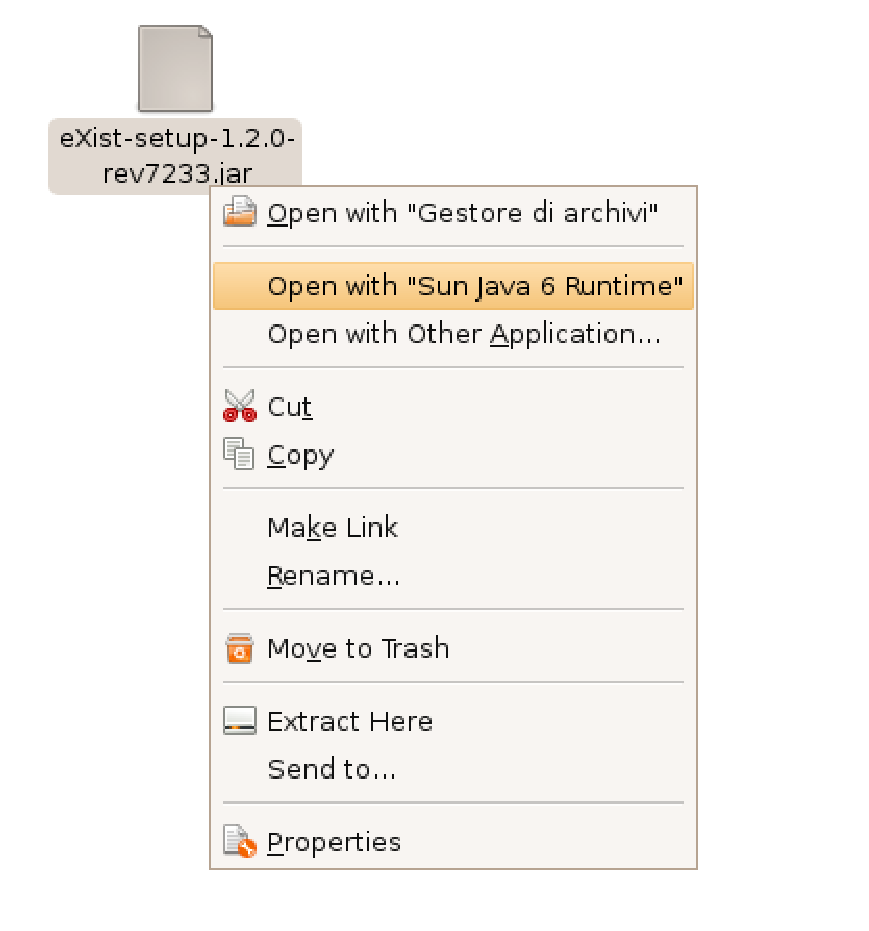
\includegraphics[width=0.5\textwidth]{manuale_utente/installazione_Exist0.eps}\\
 figura 3.1.0: come lanciare l'installazione di eXist
\end{center}
\item Comparir\`a la schermata di installazione di eXist. proseguite l'installazione premendo il tasto ``Next'' ;
\begin{center}
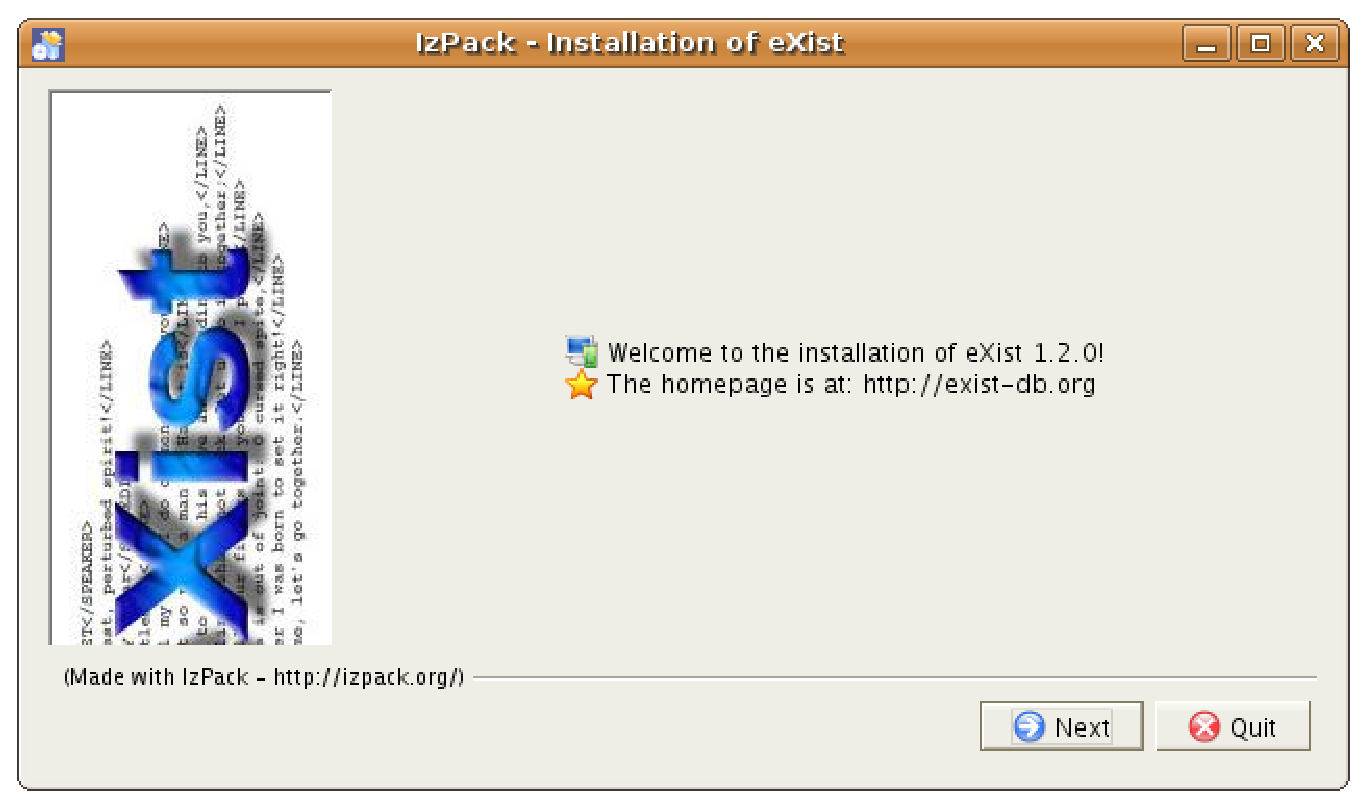
\includegraphics[width=1\textwidth]{manuale_utente/installazione_Exist1.eps}\\
 figura 3.1.1: schermata iniziale
\end{center}
\item Vi verr\`a chiesto dove installare eXist. Lasciate la directory di default (generalmente C:\textbackslash Programmi\textbackslash eXist per windows e  /home/\$USERNAME/eXist per sistemi linux). Premete il tasto ``Next'' per proseguire;
\begin{center}
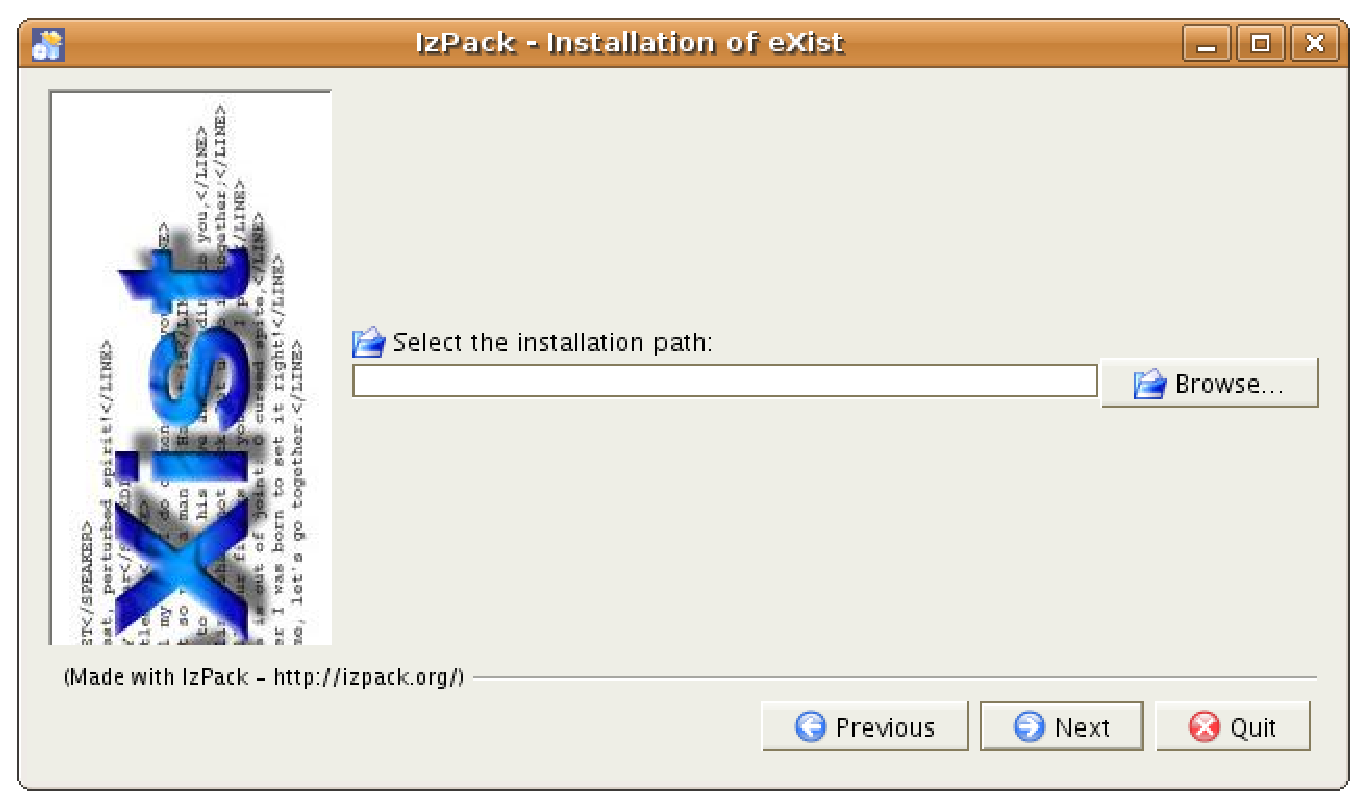
\includegraphics[width=1\textwidth]{manuale_utente/installazione_Exist3.eps}\\
 figura 3.1.2: scelta della directory
\end{center}
\item Scrivere un nome utente e una password per l'autenticazione al server DBMS negli appositi campi dati e premere sul tasto ``Next'' per proseguire. Attenzione i dati di autenticazine inseriti vi verranno richiesti all'avvio del prodotto ``Br-jsys''.
\begin{center}
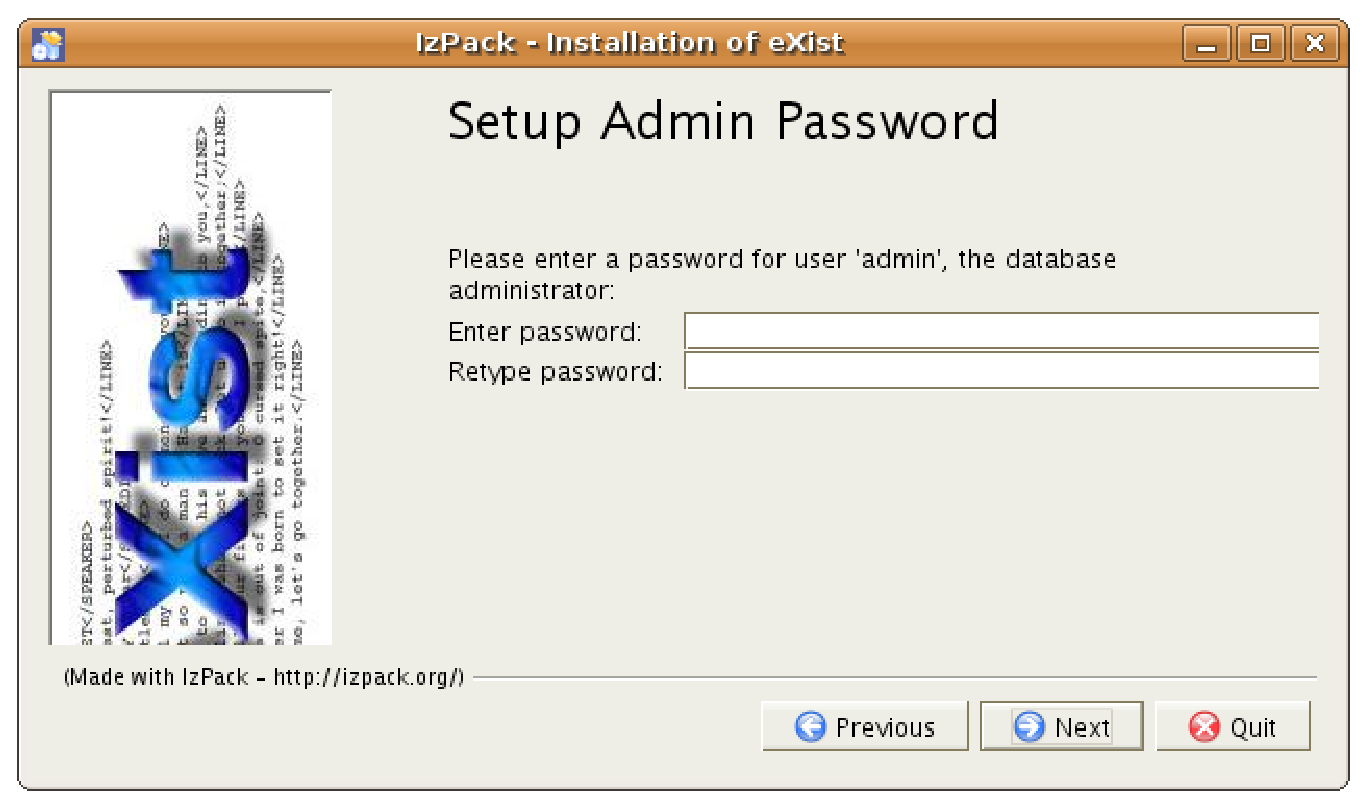
\includegraphics[width=1\textwidth]{manuale_utente/installazione_Exist4.eps}\\
 figura 3.1.3: inserimento password
\end{center}
\item Premere il tasto ``Next'' per iniziare l'installazione dei pacchetti precedentemente selezionati;
\item A questo punto \`e possibile selzionare alcune opzioni per la creazione di \textit{shortcut}. Si consiglia di mantenere la selezione di default. Premere quindi sul tasto ``Next'' per proseguire, su ``Previous'' per tornare al passo precedente o su ``Quit'' per terminare l'installazione;
\begin{center}
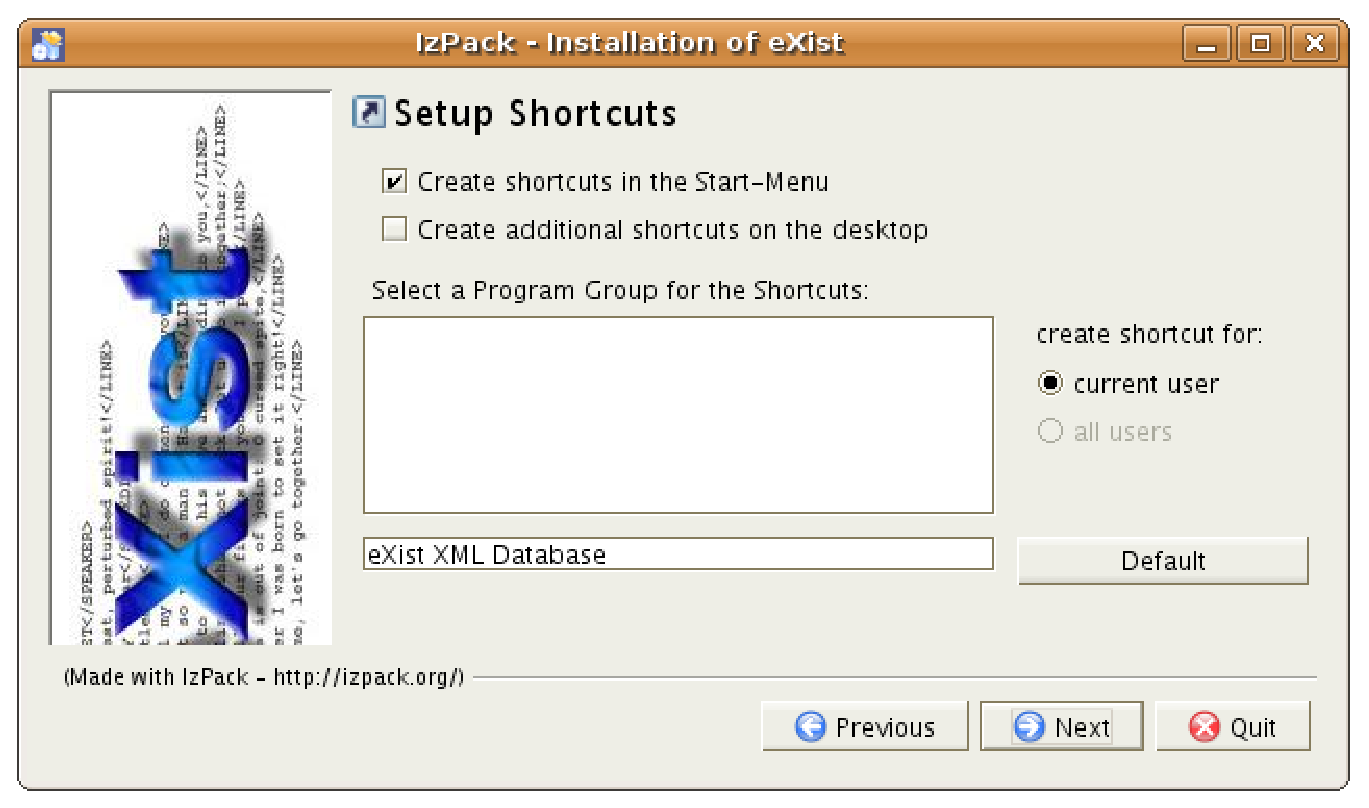
\includegraphics[width=1\textwidth]{manuale_utente/installazione_Exist6.eps}\\
 figura 3.1.4: creazione degli \textit{shortcut}
\end{center}
\item Proseguite premendo il tasto ``Next'' , fino a terminare l'installazione di eXist, verr\`a visualizzata una schermata con alcune informazioni riguardanti il prodotto. Premere su ``Quit'' per completare l'installazione;
\begin{center}
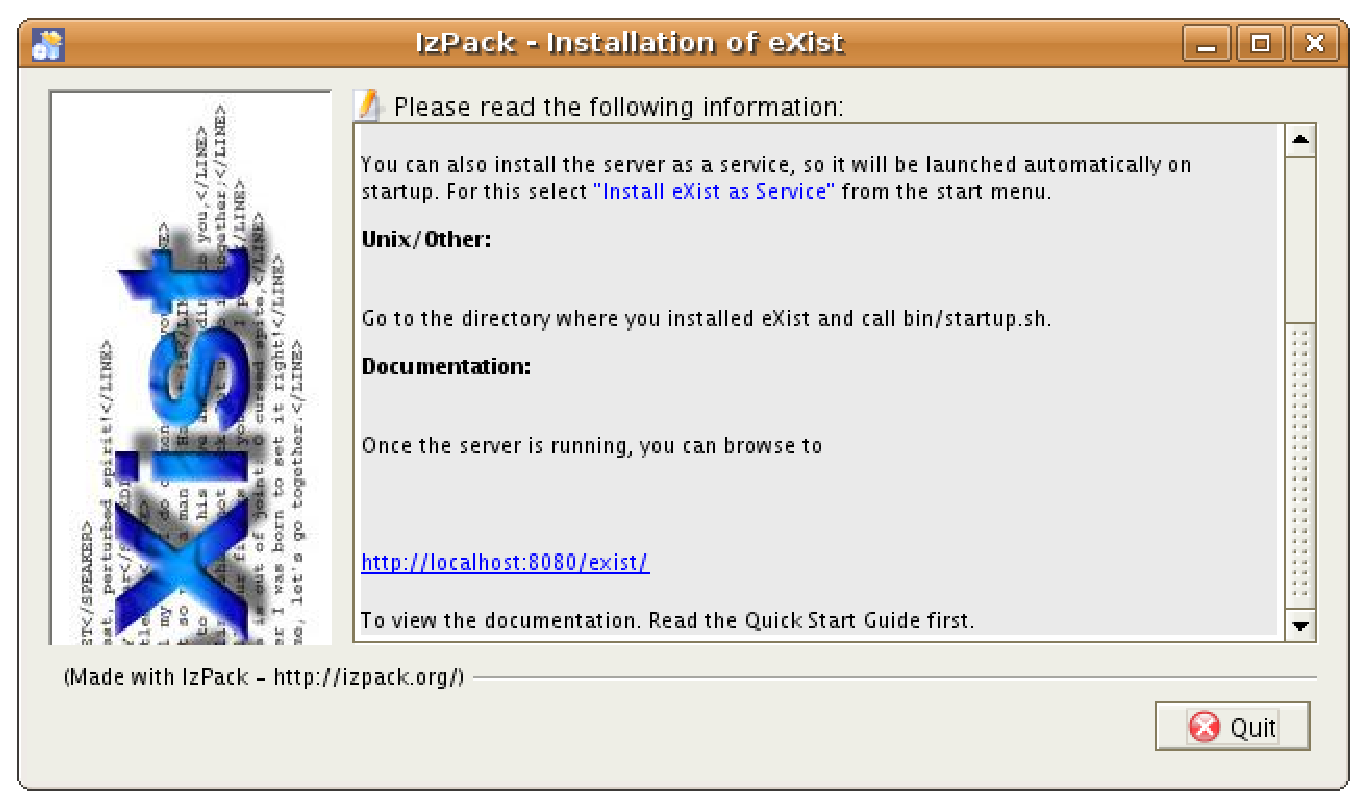
\includegraphics[width=1\textwidth]{manuale_utente/installazione_Exist8.eps}\\
 figura 3.1.5: schermata finale
\end{center}
\end{enumerate}
Per ulteriori informazioni visitare il sito\\
 \href{http://exist.sourceforge.net/quickstart.html\#sect2}{ http://exist.sourceforge.net/quickstart.html\#sect2}

\section{Installazione del prodotto}
Una volta installato eXist si pu\`o procedere con l'installazione del br-jsys.
L'installazione del prodotto segue procedure diverse da sistema operativo a sistema operativo.

\subsection{Sistemi Linux o MacOSX}
L'installazione in sistemi Linux e MacOSX avviene attraverso uno script bash. Bisogna quindi  accedere alla cartella del cd di installazione,  tramite un terminale (shell). Avviare lo script di installazione tramite il comando \textbf{sh install.sh} , il quale eseguir\`a lo script.
Lo script si occupa di psizionare corretamente i file del prodotto e di creare un link di avvio al prodotto.
Nell'illustrazione che segue potete vedere un corretto output dello script.\\
\begin{center}
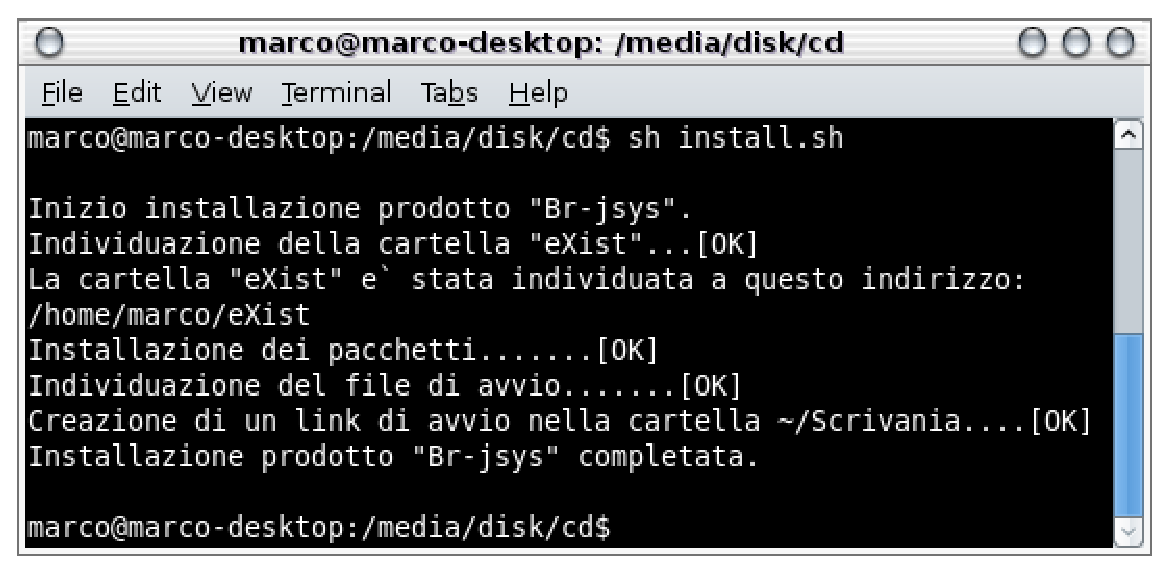
\includegraphics[width=1\textwidth]{manuale_utente/install.sh.eps}\\
 figura 3.2.1: installazione in Linux/MacOS
\end{center}

\subsection{Sistemi Windows}
L'installazione in sistemi Windows avviene attraverso un installer. Bisogna quindi accedere al cd rom di installazione e fare doppio clik sul file  \textbf{install.exe}, il quale avvier\`a un wizard di installazione.
\begin{center}
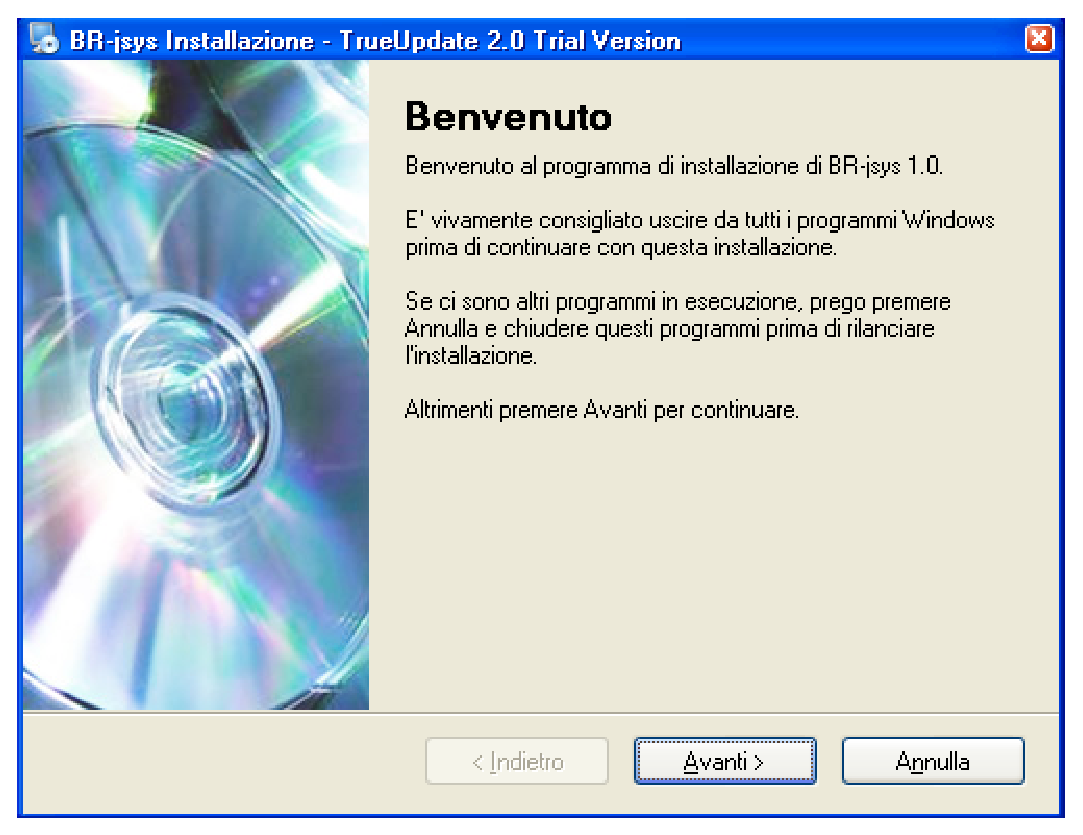
\includegraphics[width=1\textwidth]{manuale_utente/benvento.eps}\\
 figura 3.2.2: schermata iniziale in Windows
\end{center}
Leggere e seguire le istruzioni fornite dal wizard di installazione e premere il tasto ``Avanti'' per continuare.
Giunti alla schermata sottostante inserire la directory in cui installare il br-jsys (generalmente C:\textbackslash Programmi\textbackslash BR-jsys).
\begin{center}
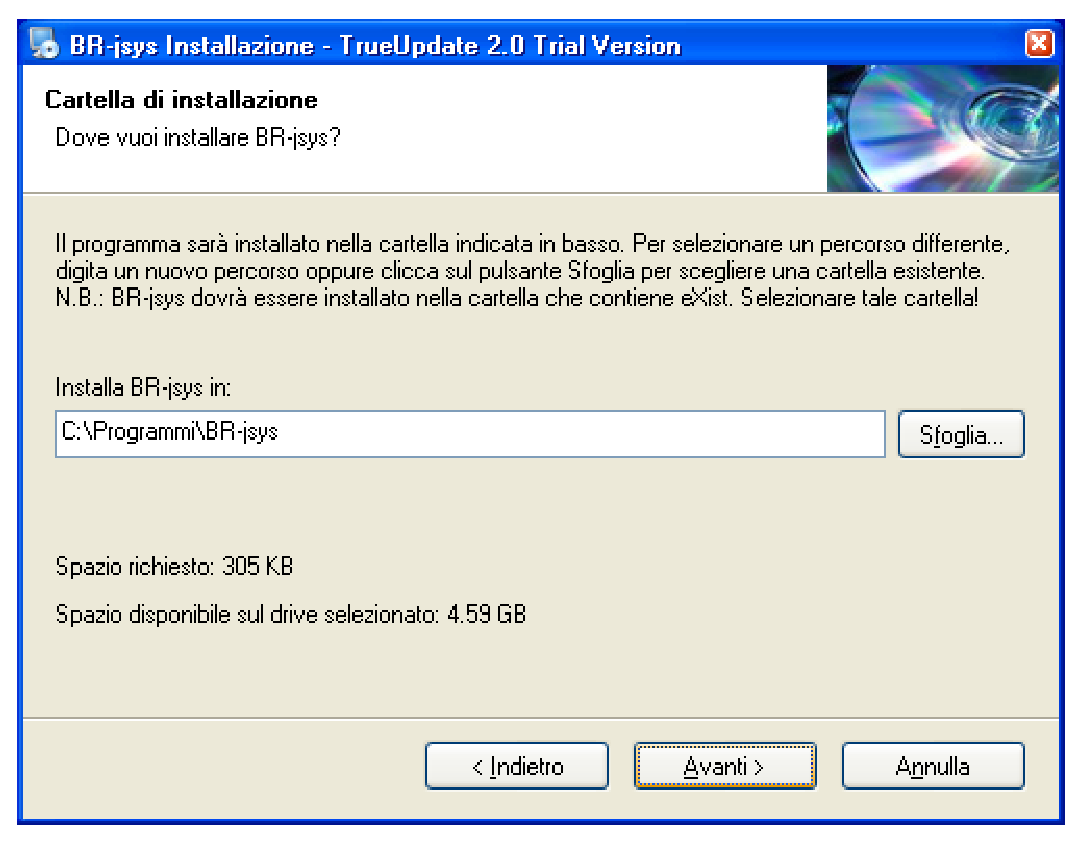
\includegraphics[width=1\textwidth]{manuale_utente/cartella_installazione.eps}\\
 figura 3.2.3: scelta della directory
\end{center}
Cliccare su ``Avanti'' finch\`e non compare la schermata di installazione completata e poi su ``Fine''.
\begin{center}
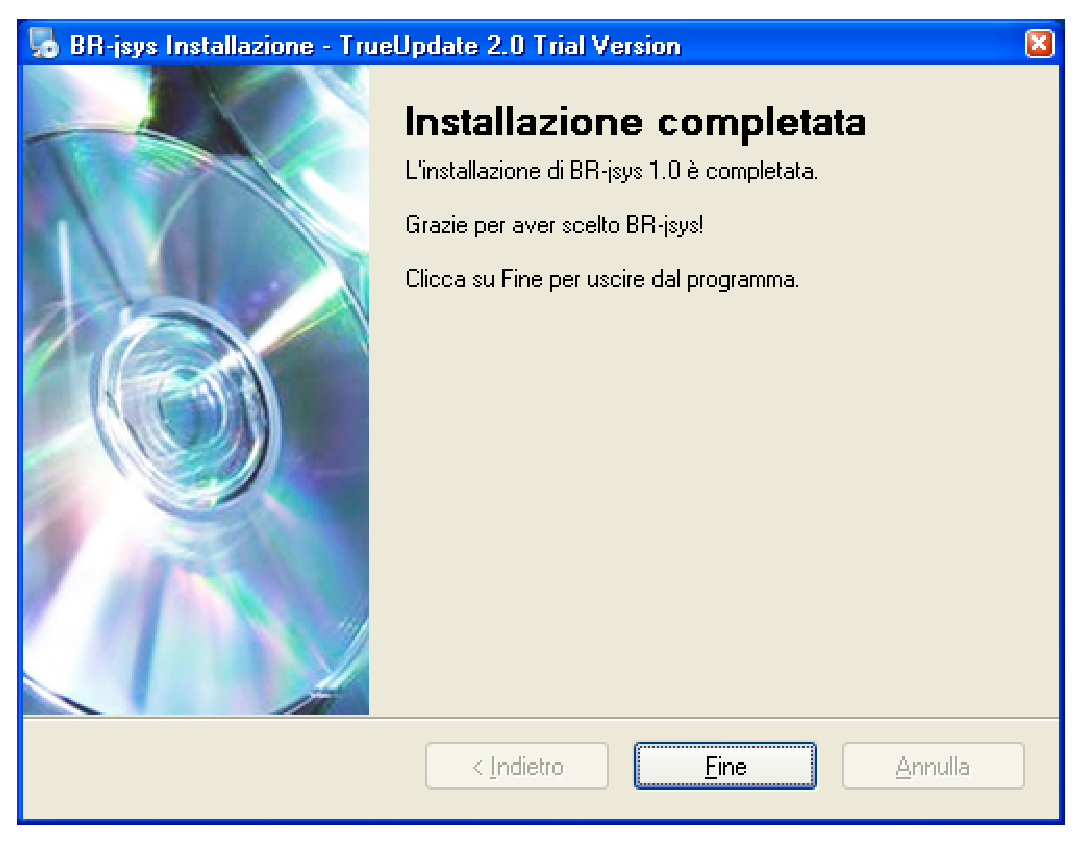
\includegraphics[width=1\textwidth]{manuale_utente/fine_installazione.eps}\\
figura 3.2.4: schermata finale
\end{center}

\chapter{Avvio del sistema}
\section{Avvio di eXist}
Perch\`e il prodotto sia avviato e funzioni correttamente \`e necessario che sia attivo il server eXist. Completata l'installazione quindi è sufficiente avviare eXist da uno degli \textit{shortcuts} creati dall'installazione. Baster\`a un doppio click sull'icona ``eXist Database Startup'' creata.\\
Per lanciare eXist manualmente:
\begin{itemize}
\item[1-] Aprire la shell di Linux o il prompt dei comandi (Dos) di Windows;
\item[2-] Accedere alla directory in cui \`e installato eXist e successivamente dentro la cartella `bin';
\item[3-] Da shell di Linux digitate:  \textbf{startup.sh} . Dal prompt dei comandi di Windows digitate: \textbf{startup.bat};
\end{itemize}	
Apparir\`a cos\`i una schermata simile alla seguente.
\begin{center}
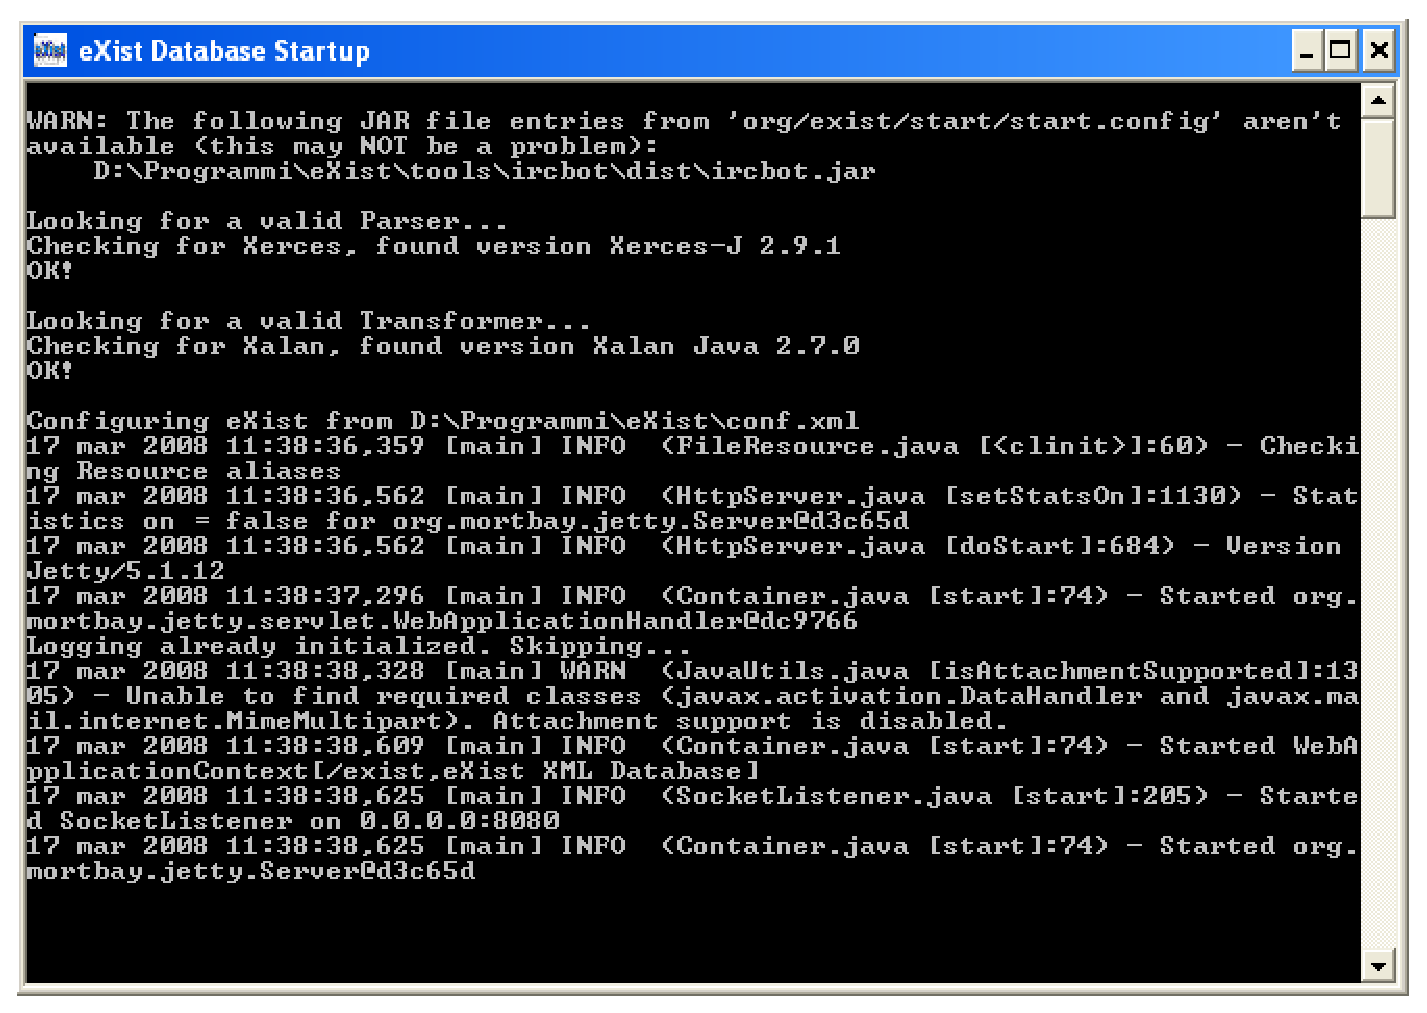
\includegraphics[width=1\textwidth]{manuale_utente/avvio-exist.eps}\\
figura 3.4.1: schermata di avvio di eXist
\end{center}
Per ulteriori informazioni visitare il sito\\
 \href{http://exist.sourceforge.net/quickstart.html\#sect3}{ http://exist.sourceforge.net/quickstart.html\#sect3}


\section{Avvio dell'applicazione}
Per avviare il programma, una volta terminato l'avvio del server eXist, bisogna:
\begin{itemize}
 \item Nei sitemi Linux cliccare col tasto destro del mouse su brjsys.jar e selezionare ``apri con Java 6 Runtime Environment''
\item Nei sistemi Windows accedere alla cartella in cui si installato il prodotto (generalmente \texttt{C:\textbackslash Programmi\textbackslash BR-jsys} ) e fare doppio click su brjsys.jar 
\end{itemize}
Apparir\`a la schermata di login (figura 4.2.0), nella quale l'utente dovr\`a inserire l'\textit{username} e la \textit{password} di connessione a eXist.
\begin{center}
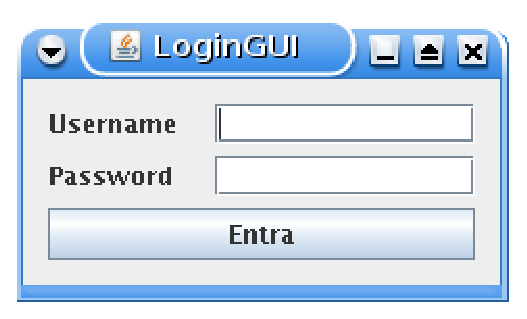
\includegraphics[width=0.5\textwidth]{manuale_utente/login.eps}\\
 figura 4.2.0: schermata di login
\end{center}
I dati di autenticazione da immettere sono quelli utilizzati per la registrazione al server ``\underline{eXist}''.
In caso di login eseguito correttamente, verr\`a lanciata la schermata principale (figura 4.2.1).
\begin{center}
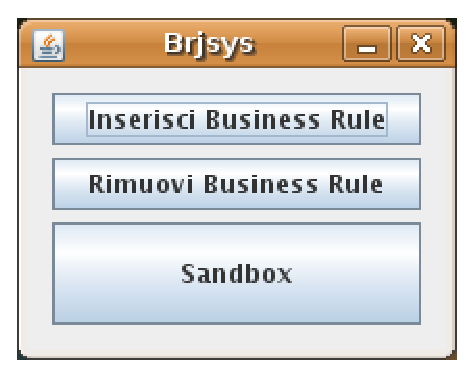
\includegraphics[width=0.5\textwidth]{manuale_utente/schermata_principale.eps}\\
 figura 4.2.1: schermata principale corretamente avviata
\end{center}
Se eXist non \`e stato avviato correttamente o pi\`u semplicemente non \`e stato avviato, verr\`a mostrato all'utente un messaggio di errore indicando che il server eXist \`e spento (figura 4.2.2). \`E necessario quindi chiudere il prodotto avviare il server eXist e riavviare il ``Br-jsys''.
\begin{center}
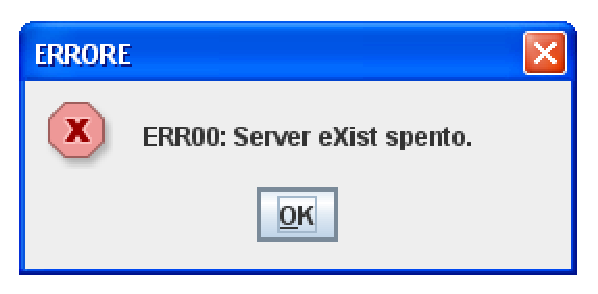
\includegraphics[width=0.7\textwidth]{manuale_utente/errore_server_spento.eps}\\
 figura 4.2.2: esempio di server spento
\end{center} 
Se l'username e la password non sono stati inseriti correttamente verr\`a mostrato un messaggio d'errore (figura 4.2.3). Reinserite quindi username e password corretti.
\begin{center}
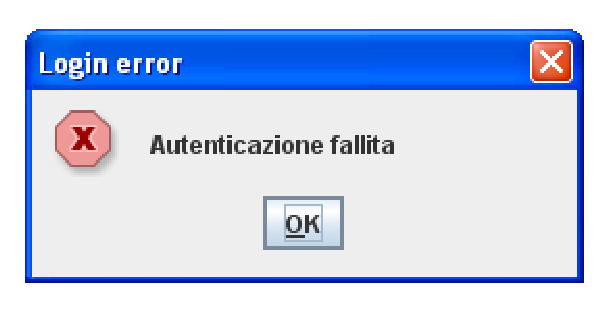
\includegraphics[width=0.7\textwidth]{manuale_utente/autenticazione_fallita.eps}\\
figura 4.2.3: esempio di username e/o password errati
\end{center}

\chapter{Funzionalit\`a del sistema}
\section{Descrizione funzionale}
Di seguito \`e riportata la descrizione delle funzioni del prodotto. Ad ogni passo \`e stata associata una figura, in modo da daterminare senza amibiguit\`a il contesto dell'applicazione. Una volta avviato il prodotto ed essersi autenticati presso il DBMS verr\`a visualizzata la schermata principale (vedi figura 4.2.1).
Da questa schermata si possono avviare le tre funzionalit\`a associate ai rispettivi bottoni:
\begin{itemize}
\item Inserisci \br;
\item Rimuovi \br;
\item Sandbox.
\end{itemize}
Per ottenere maggiori informazioni sul prodotto viene messo a disposizione un ``Help'' raggiungibile dal Men\`u (figura 5.1.0), dal quale si potr\`a consultare il Manuale e il Javadoc.
\begin{center}
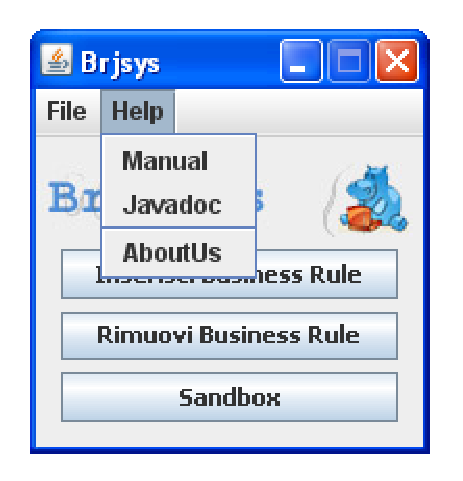
\includegraphics[width=0.5\textwidth]{manuale_utente/schermata_help.eps}\\
 figura 5.1.0: Help
\end{center}
Se l'utente cerca di consultare il Manuale o il Javadoc ma essi risultano assenti, verranno sollevati i seguenti errori.
\begin{center}
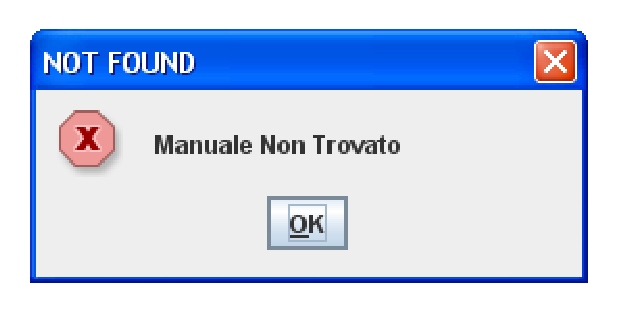
\includegraphics[width=0.7\textwidth]{manuale_utente/errore_manuale.eps}\\
figura 5.1.1: esempio di Manuale non trovato
\end{center}
\begin{center}
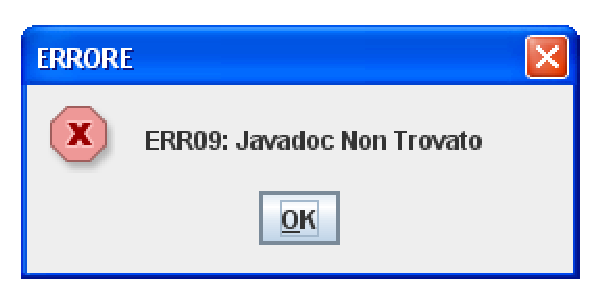
\includegraphics[width=0.7\textwidth]{manuale_utente/errore_javadoc.eps}\\
figura 5.1.2: esempio di Javadoc non trovato
\end{center}
L'analisi dettagliata delle singole azioni verr\`a trattata nelle sezioni seguenti.
\section{Inserisci \br}
\begin{center}
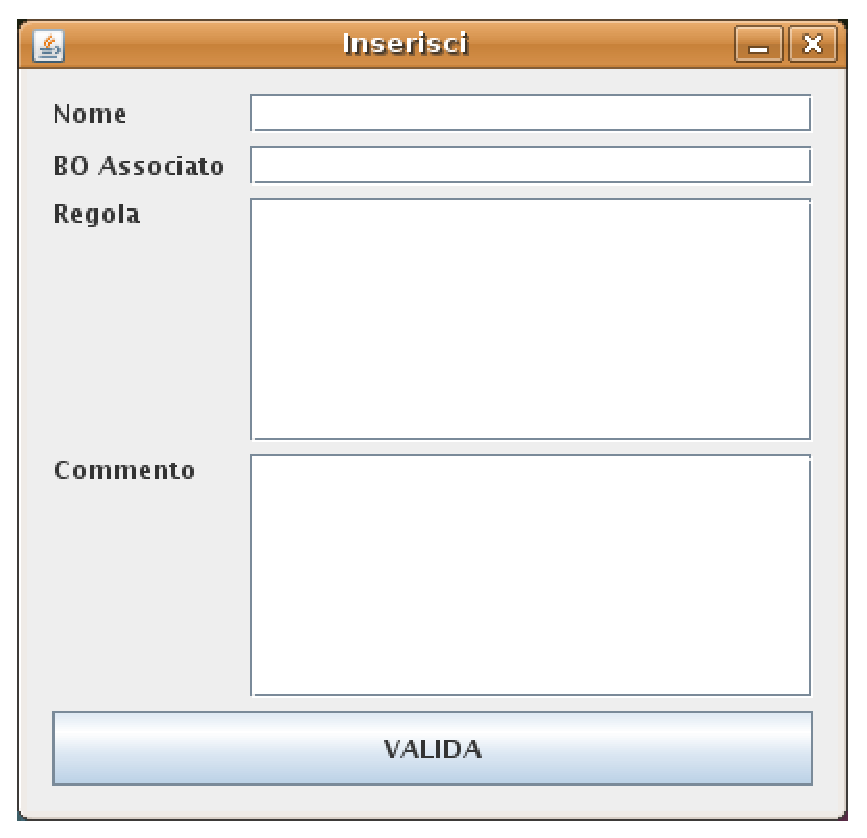
\includegraphics[width=1\textwidth]{manuale_utente/schermata_inserimento.eps}\\
 figura 5.2.0: schermata di inserimento
\end{center}
Nella figura 5.2.0 vediamo illustrata la schermata di inserimento di una nuova \br. Per inserire una nuova \br\ e popolare quindi il database bisogna inserire negli appositi spazi i campi dati richiesti.
Nel campo ``Regole Presenti'' l'utente pu\`o ricercare le \br gi\`a presenti nel repository.
\subsection{Nome}
Il nome della \br\ che l'utente intende inserire. Il nome della \br\ deve essere univoco all'interno del \rp. Per questo motivo \`e importante prestare attenzione al nome scelto. \`E consigliabile definire all'interno dell'azienda che utilizza il prodotto delle regole di nomenclatura per il nome delle \br. Per facilitare un corretto inserimento della \br\ \`e presente una lista delle \br\ inserite nel \rp. \`E cos\`i possibile visualizzare in modo rapido le \br\ gi\`a inseirte evitando di inseire una \br\ con un nome gi\`a inseirto nel \rp.

\subsection{Business Object Associato}
Il \bo\ al quale si vuole associare la regola. Il linguaggio di definizione delle \br\ offre la possibilit\`a di effettuare operazioni e controlli sui campi dati dei \bo\ da validare. Per questo ad ogni \br\ \`e necessario associare un \bo. Per facilitare l'inserimento di una nuova \br\ (evitando cos\`i errori dovuti ad una digitazione errata del nome del \bo) il campo \bo\ associato \`e una \textit{combobox} che permette di scegliere uno dei \bo\ realmente presenti.

\subsection{Regola}
La regola scritta secondo la grammatica spiegata nel capitolo `Descrizione del Linguaggio'. Per ovviare all'inserimento di \br\ con il campo regola identico, \`e possibile selezionare una delle \br\ della lista e visualizzare il campo `regola' nella \textit{statusbar} figura 5.2.3.

\begin{center}
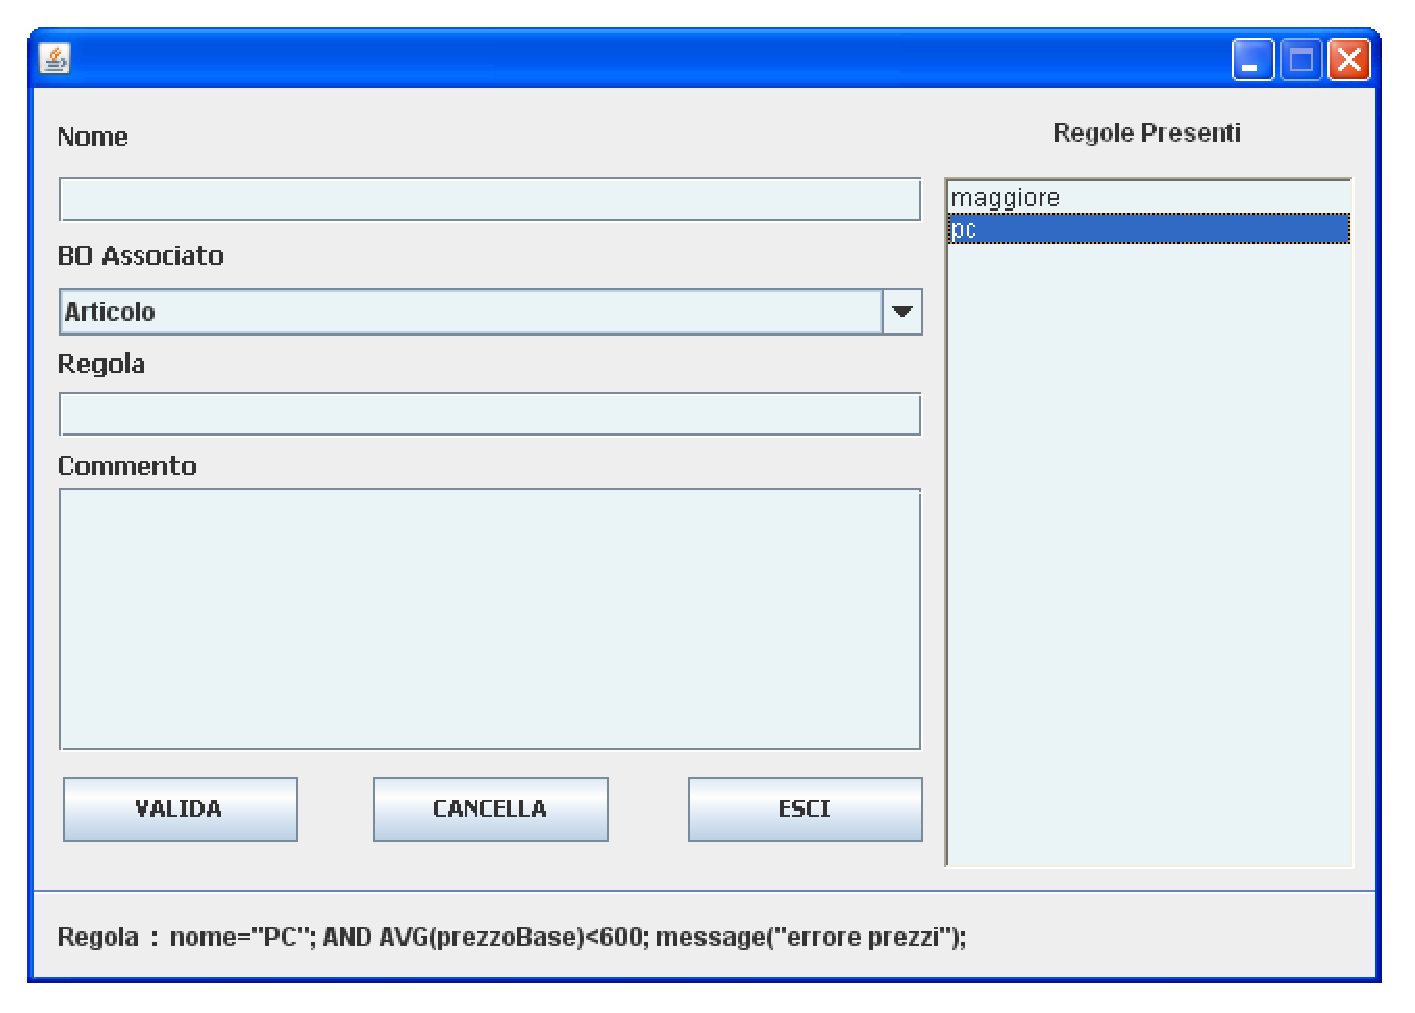
\includegraphics[width=1\textwidth]{manuale_utente/schermata_esempio_regola_selezionata.eps}\\
 figura 5.2.3: campo dati regola selezionata
\end{center} 

\subsection{Commento}
Descrizione sintetica del comportamento della regola. Il commento \`e opzionale e serve a fornire una descrizione pi\`u chiara e leggibile della regola stessa.

\subsection{Validazione e inserimento}
L'utente dovr\`a poi cliccare sul pulsante ``\textbf{Valida}''. Se l'inserimento viene effettuato con successo verr\`a visualizzato un messaggio di conferma. In caso contrario un messaggio d'errore indicher\`a all'utente cosa va modificato nella \br\ affinch\`e venga validata correttamente. In alternativa potr\`a cliccare sul tasto ``Cancella'' per rimuovere i dati immessi.
\begin{center}
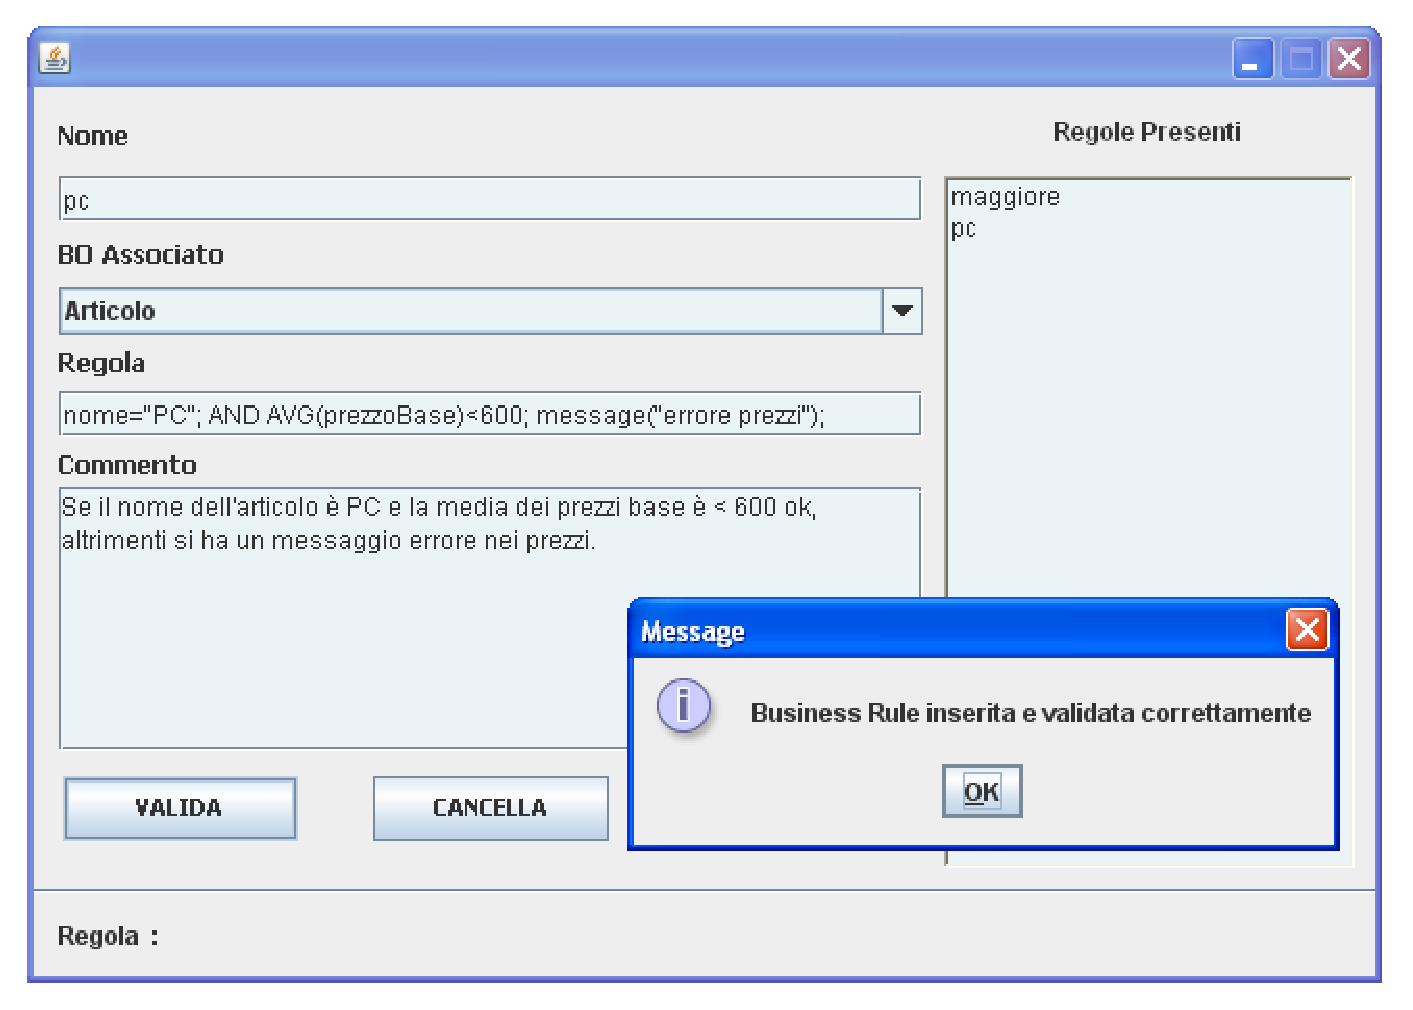
\includegraphics[width=1\textwidth]{manuale_utente/schermata_esempio_inserimento.eps}\\
 figura 5.2.5: esempio di inserimento
\end{center} 
\subsection{Esiti}
\begin{center}
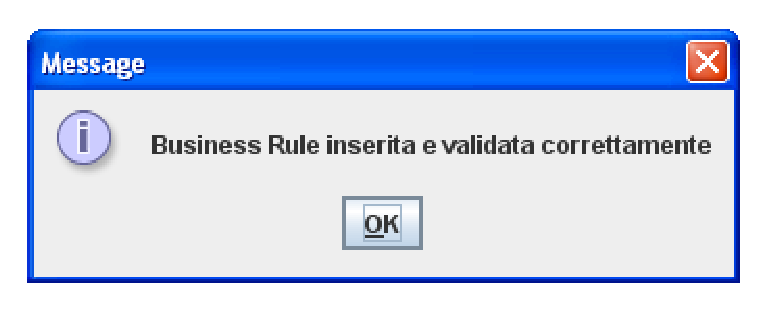
\includegraphics[width=0.7\textwidth]{manuale_utente/br_inserita.eps}\\
 figura 5.2.6: esempio inserimento effettuato
\end{center} 
La figura 5.2.6 mostra l'esito di un corretto inserimento di una \br. La \br\ \`e stata cos\`i validata e inserita nel \rp.

\begin{center}
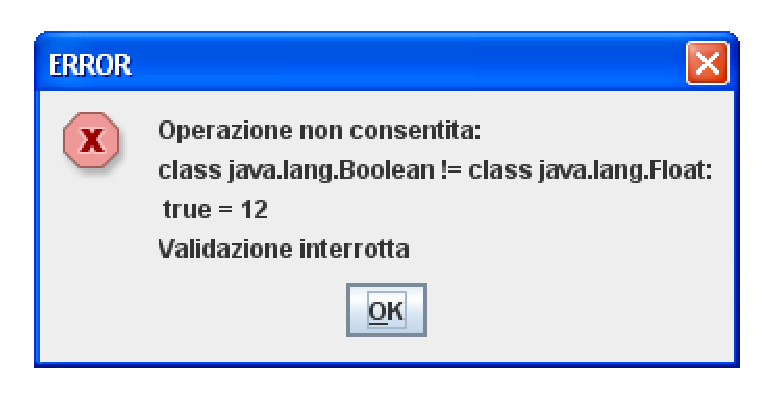
\includegraphics[width=0.7\textwidth]{manuale_utente/errore_op_non_consentita.eps}\\
 figura 5.2.6.1: esempio di regola sintatticamente errata 
\end{center} 
La figura 5.2.6.1 mostra l'esito di un errato inserimento di business rules. La business rule non pu\`o essere validata e inserita nel \rp\ in quanto la regola immessa (in questo caso true=12) non \`e consentita.
\\
\\
\begin{center}
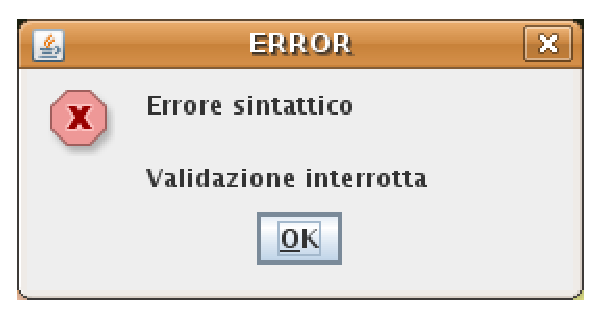
\includegraphics[width=1\textwidth]{manuale_utente/errore_sintattico.eps}\\
 figura 5.2.6.2: esempio di regola errata
\end{center} 
La figura 5.2.6.2 mostra l'esito di un errato inserimento di business rules. La business rule non pu\`o essere validata e inserita nel \rp\ in quanto la regola immessa \`e scritta in maniera errata.

\begin{center}
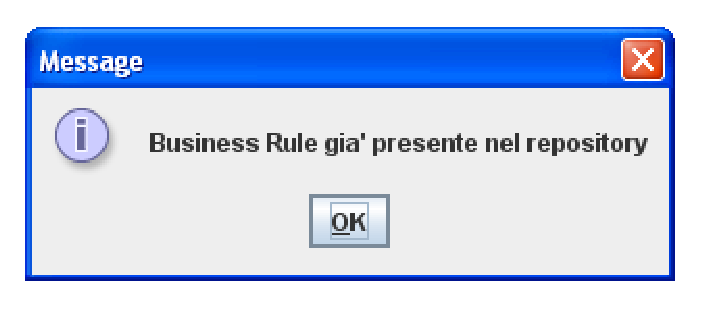
\includegraphics[width=0.7\textwidth]{manuale_utente/errore_br_gia_presente.eps}\\
 figura 5.2.6.3: esempio di regola gi\`a inserita
\end{center} 
La figura 5.2.6.3 mostra l'esito di un errato inserimento di business rules. La business rule non pu\`o essere validata e inserita nel \rp\ in quanto vi \`e gi\`a un'occorrenza di questa nel \rp. In questo caso viene selezionata la \br\ trovata nella lista ``Regole Presenti'' e visualizzato il corrispondente campo `regola' nella \textit{statusbar}.

\begin{center}
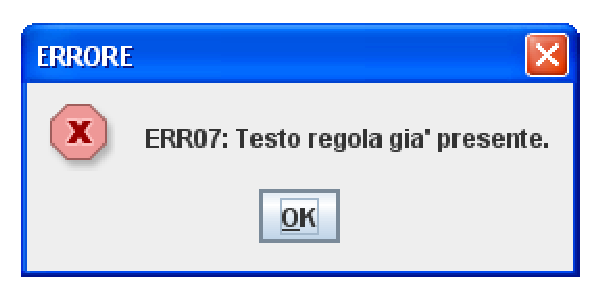
\includegraphics[width=0.7\textwidth]{manuale_utente/errore_testo_gia_presente.eps}\\
 figura 5.2.6.4: esempio testo regola gi\`a presente
\end{center} 
La figura 5.2.6.4 mostra l'esito di un errato inserimento di \underline{business rules}. La business rule non pu\`o essere validata e inserita nel \rp\ in quanto vi \`e gi\`a un \br\ con quel campo . In questo caso viene selezionata tale \br\ nella lista ``Regole Presenti'' e visualizzato il corrispondente campo `regola' nella \textit{statusbar}.

\begin{center}
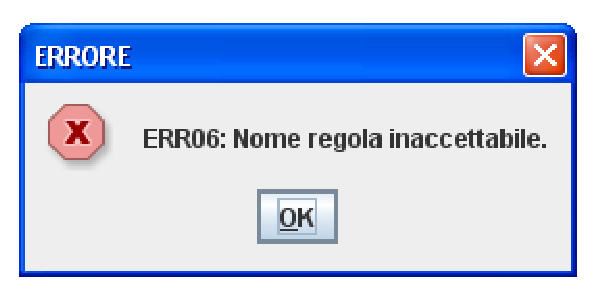
\includegraphics[width=0.7\textwidth]{manuale_utente/errore_nome_regola_inaccettabile.eps}\\
 figura 5.2.6.5: esempio inserimento nome vuoto
\end{center} 
La figura 5.2.6.5 mostra l'esito di un errato inserimento di business rules. La business rule non pu\`o essere validata e inserita nel \rp\ in quanto il nome inserito  della \br\ \`e vuoto.

\begin{center}
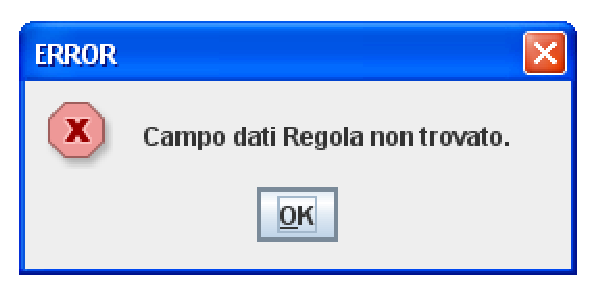
\includegraphics[width=0.7\textwidth]{manuale_utente/errore_campodati.eps}\\
 figura 5.2.6.6: esempio inserimento campo dati non presente nel business object associato
\end{center} 
La figura 5.2.6.6 mostra l'esito di un errato inserimento di business rules. La business rule non pu\`o essere validata e inserita nel \rp\ in quanto il campo dati della \br\ non \`e presente nel business object associato.


\section{Rimuovi \br}
\begin{center}
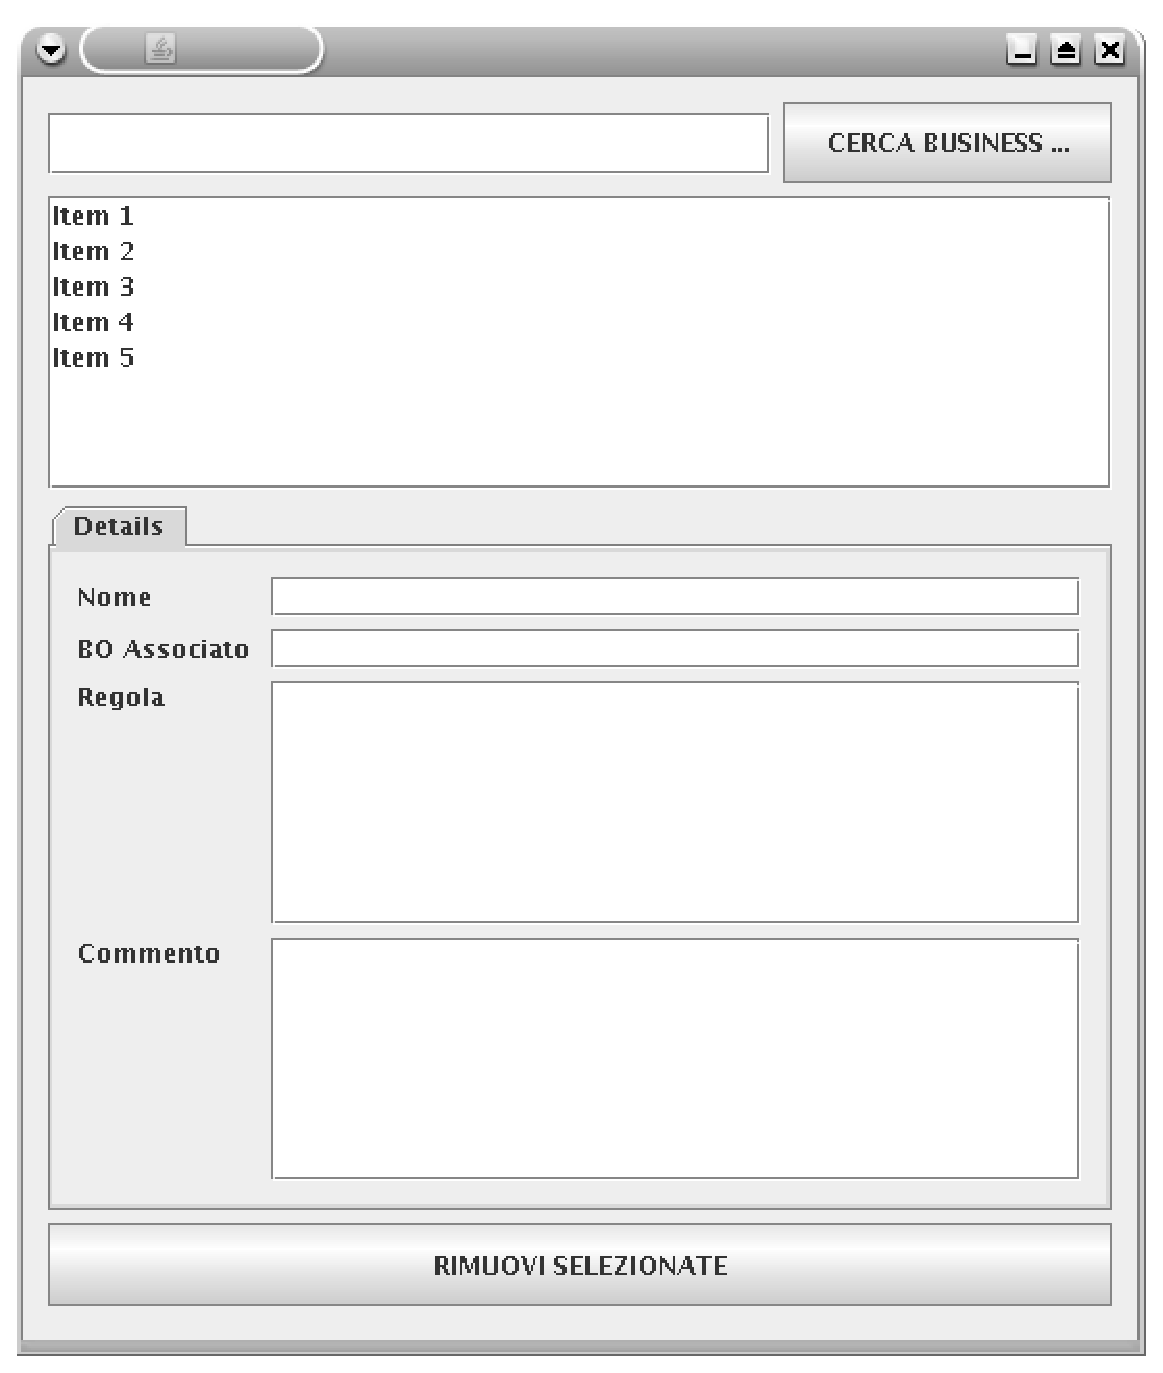
\includegraphics[width=1\textwidth]{manuale_utente/schermata_rimozione.eps}\\
 figura 5.3.0: schermata di rimozione
\end{center}
Nella figura 5.3.0 vediamo illustrata la schermata di cancellazione di una business rule.
\begin{itemize}
\item Per procedere all'eliminazione l'utente avr\`a 2 modi:
\begin{enumerate}
\item inserire nell'appostito campo (TextBox) il nome della business rule si che intende rimuovere e cliccare sul pulsante ``\textbf{Cerca}''. Se l'utente opera una o pi\`u ricerche, le \br\ trovate verranno selezionate nel campo ``Business Rules Selezionate'' mentre in ``Lista Completa'' sar\`a evidenziata solo l'ultima di queste. Si possono eventualmente deselezionare le \br\ attraverso il tasto ``Deseleziona''. Viene infine introdotto l'uso di espressioni regolari per raffinare la ricerca, in questo caso invitiamo l'utente a consultare la documentazione fornita all' url:\\ \href{http://java.sun.com/j2se/1.4.2/docs/api/java/util/regex/Pattern.html}{http://java.sun.com/j2se/1.4.2/docs/api/java/util/regex/Pattern.html}.
\item selezionare una o pi\`u \underline{business rule} dalle liste sottostanti.
\end{enumerate}

\item Se la \underline{business rule} risulta presente nel \rp\, comparir\`a  nel campo ``Details'' i suoi dettagli (Nome, BO Associato, Regola, Commento) figura 5.3.0.1. 

\begin{center}
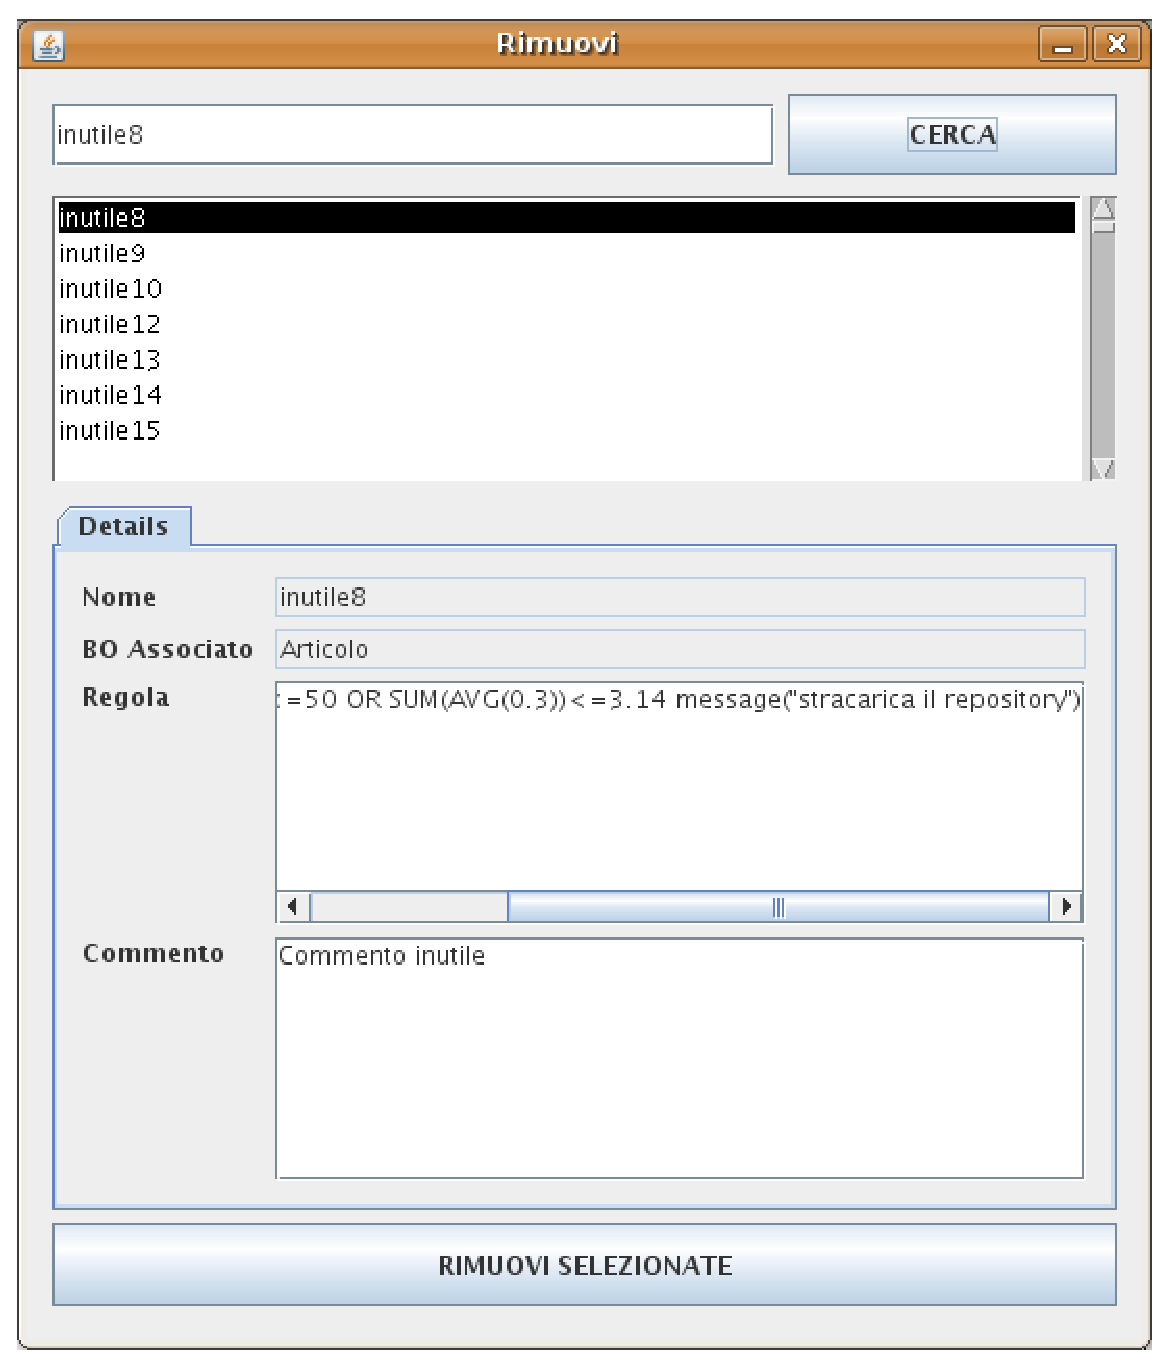
\includegraphics[width=1\textwidth]{manuale_utente/rimozione_br_trovata.eps}\\
 figura 5.3.0.1: esempio di regola selezionata.
\end{center} 

\begin{center}
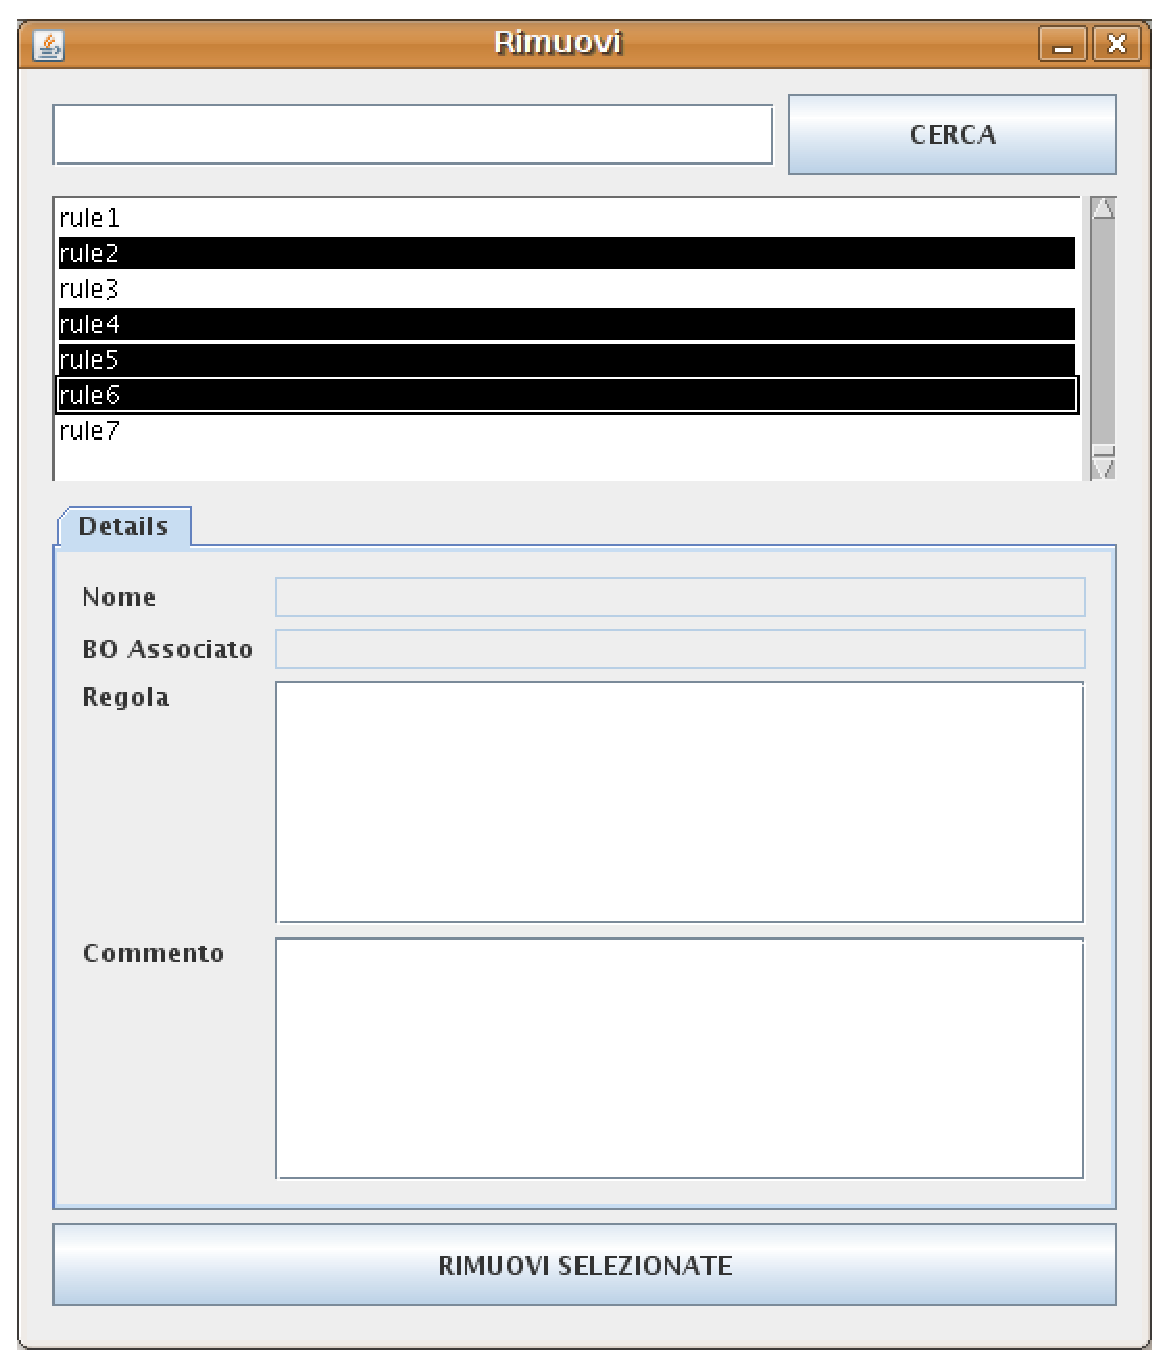
\includegraphics[width=1\textwidth]{manuale_utente/selezione_multipla.eps}\\
 figura 5.3.0.2: esempio di selezione multipla.
\end{center} 

\begin{center}
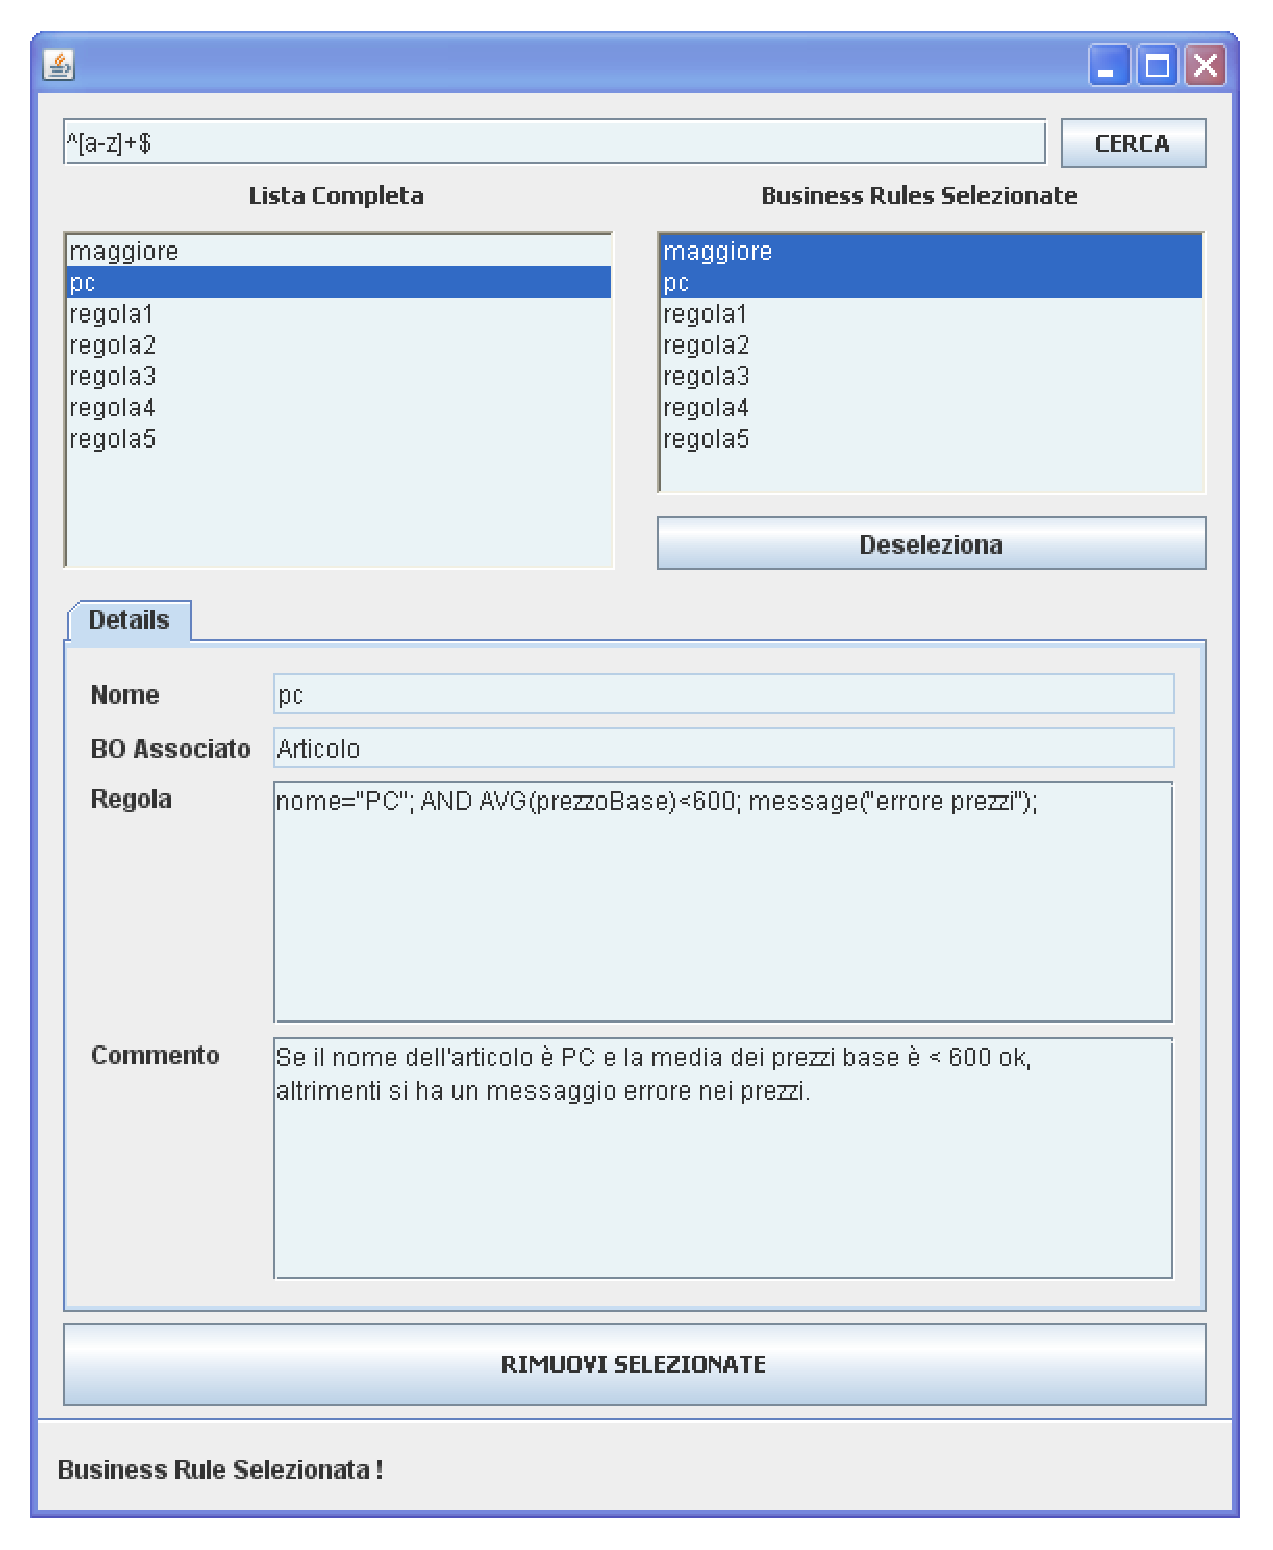
\includegraphics[width=1\textwidth]{manuale_utente/schermata_rimozione_multipla.eps}\\
 figura 5.3.0.3: esempio di selezione con espressioni regolari.
\end{center} 

\item A questo punto baster\`a cliccare sul pulsante ``\textbf{Rimuovi Selezionate}'' e dare conferma di rimozione figura 5.3.0.4  
\end{itemize}

\begin{center}
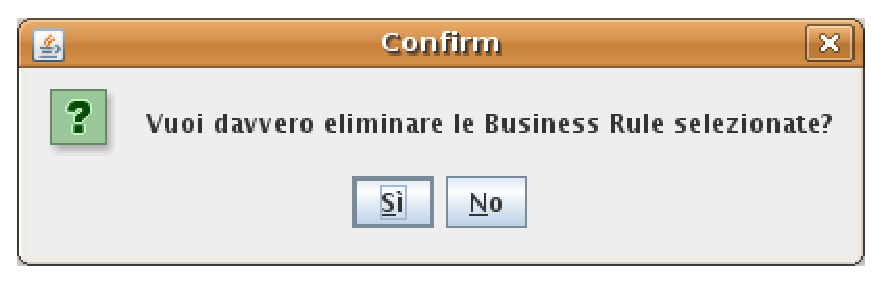
\includegraphics[width=0.7\textwidth]{manuale_utente/conferma_rimozione.eps}\\
 figura 5.3.0.4 messaggio di conferma.
\end{center} 

Se la cancellazione viene effettuata con successo verr\`a visualizzato un messaggio nella \textit{statusbar} che ne conferma l'esito positivo, in caso contrario uno negativo.
\subsection{Esiti}
 
\begin{center}
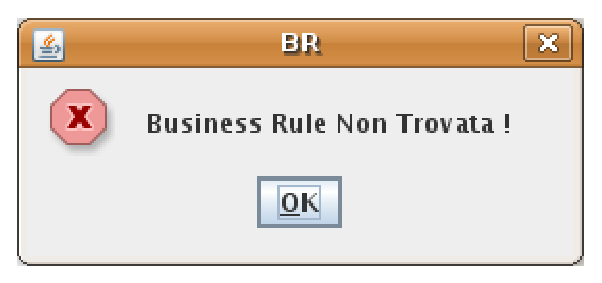
\includegraphics[width=0.7\textwidth]{manuale_utente/br_non_trovata.eps}\\
 figura 5.3.1 messaggio di regola non trovata.
\end{center} 
La figura 5.3.1 mostra l'esito di un'errata rimozione di business rules. La business rule non pu\`o essere rimossa dal \rp\ in quanto non \`e stata trovata al suo interno.

\begin{center}
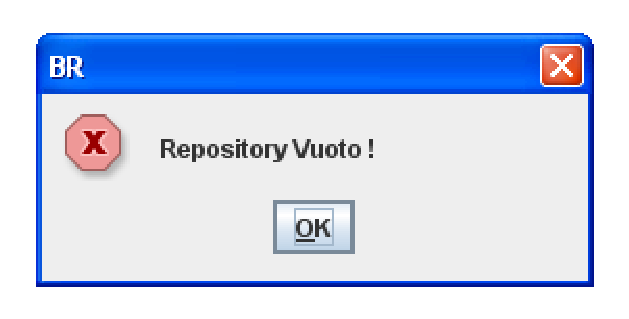
\includegraphics[width=0.7\textwidth]{manuale_utente/errore_repository_vuoto.eps}\\
 figura 5.3.2 messaggio di repository vuoto.
\end{center} 
La figura 5.3.2 mostra l'esito di un'errata rimozione di business rules. La business rule non pu\`o essere rimossa dal \rp\ in quanto il repository non ne contiene alcuna.

\section{Sandbox}
\begin{center}
 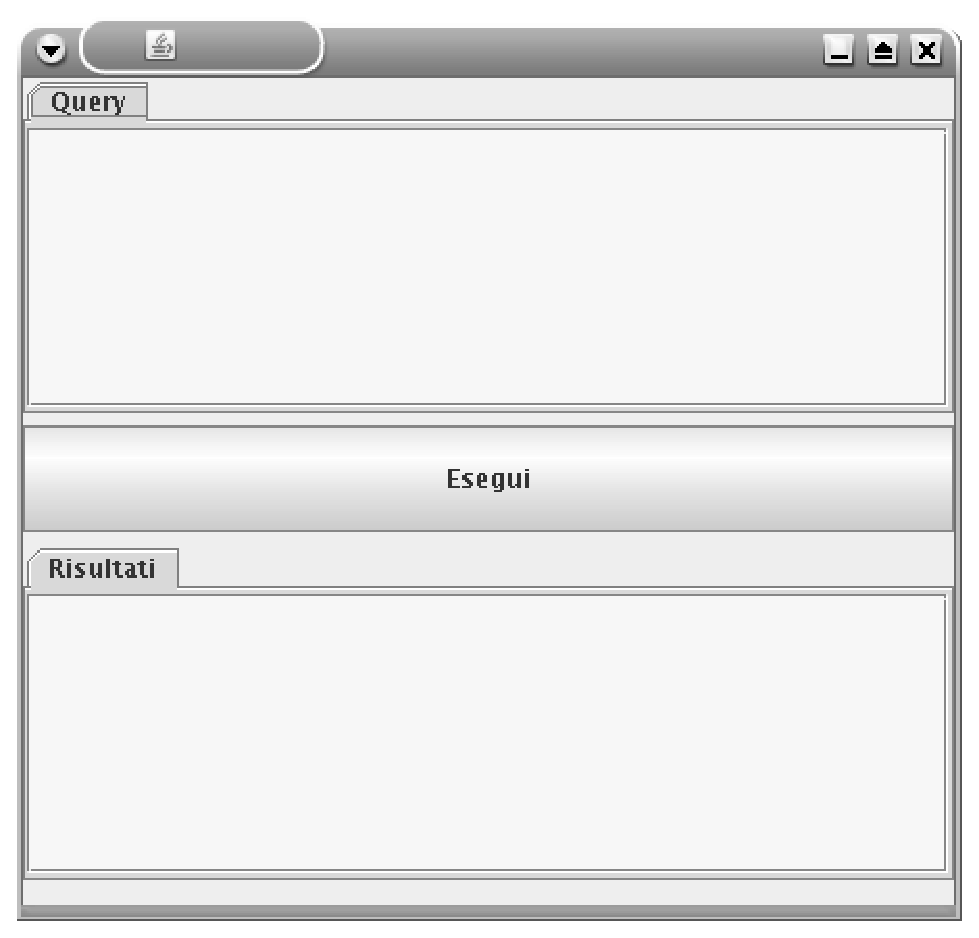
\includegraphics[width=1\textwidth]{manuale_utente/schermata_sandbox.eps} \\
 figura 5.4: schermata sandbox
\end{center}
Nella figura 5.4 vediamo illustrata la schermata di \underline{sandbox}. Per procedere con l'interrogazione del DBMS, l'utente dovr\`a:
\begin{itemize}
\item inserire la query (scritta in linguaggio \underline{XQuery}) nell'appostito campo dati ``Query'';
\item cliccare sul pulsante ``\textbf{Esegui}''.
\item cliccare sul pulsante ``\textbf{Cancella}'' se invece si vuole cancellare il testo della query scritta.
\end{itemize}

\subsection{Esiti}
\begin{center}
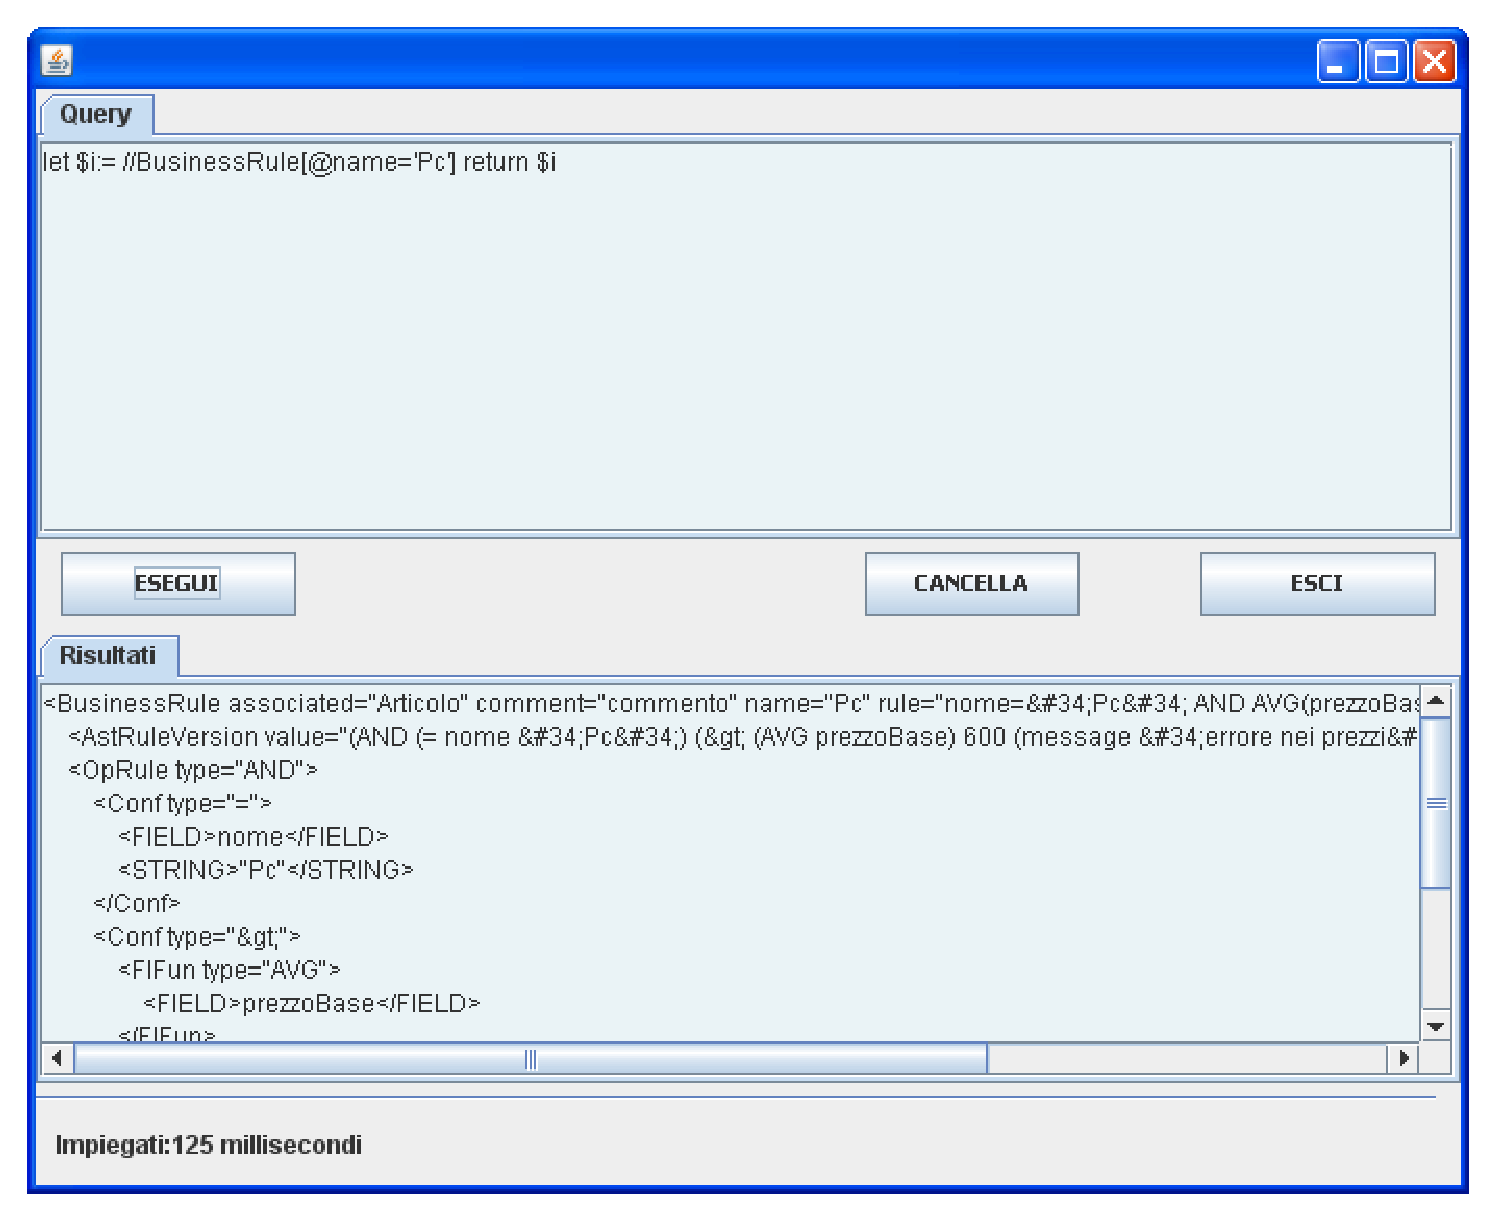
\includegraphics[width=1\textwidth]{manuale_utente/sandbox_di_query.eps}\\
 figura 5.4.1 esempio di querying corretto.
\end{center}
La figura 5.4.1 mostra l'esito positivo di una query e in particolare verr\`a visualizzato nel campo dati ``Risultati'' l'esito della query e nella barra sottostante il tempo di risposta (in millisecondi) impiegato da eXist.

\begin{center}
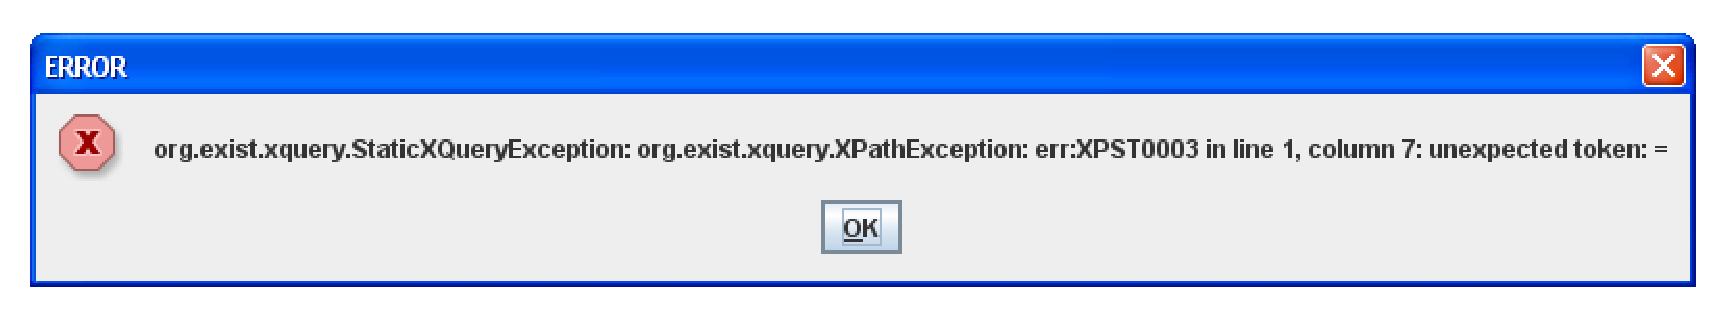
\includegraphics[width=0.7\textwidth]{manuale_utente/esempio_errore_sandbox_query_errata.eps}\\
figura 5.4.2 Inserimento query errata.
\end{center}
La figura 5.4.2 mostra un'eccezione lanciata in caso di esito negativo di una query scritta in maniera errata.


\chapter{Descrizione del linguaggio}
In questo capitolo viene descritto il linguaggio di formulazione di \br. Una \br\ serve a definire vincoli e regole da rispettare per un determinato \bo. Per questo il linguaggio di definizione delle \br\ \`e incentrato soprattutto sul confronto tra campi dati dei \bo\ ed espressioni algebrica o valori costanti. In una \br\ quindi si possono ottenere valori attraverso l'utilizzo di espressioni algebriche, definire confronti tra questi valori e campi dati dei \bo\ e collegare questi confronti con operatori logici. L'insieme delle funzionalit\`a del linguaggio garantisce una buona espressivit\`a.
\`E molto importante chiarire l'utilizzo delle \br. Le \br\ sono concepite per verificare che un oggetto rispetti determinati vincoli. I vincoli che si definiscono con una \br\ sono vincoli oggettivi ad esempio ``\texttt{se un valore è maggiore di 10 non deve essere minore di 10}'' e non vincoli soggettivi come ``\texttt{le entrate devono essere maggiori delle uscite}'' mentre per la prima regola non \`e possibile che avvenga il contrario, per la seconda ci\`o \`e possibile per quanto negativo possa essere per una azienda.

\section{Una \br\ semplice}
Una \br semplice \`e costituita da un singolo confronto. Ad esempio: ``prezzo\textgreater0;'' . La regola appena scritta serve a verificare che ogni oggetto abbia un prezzo maggiore di zero. Nella regola ``prezzo'' \`e il nome di un campo dati dell'oggetto. Una regola minimale \`e quindi definita dal comfronto tra un campo dati dell'oggetto e un valore. \\
Ogni confronto va terminato da un ``;''. \\
Gli operatori di confronto ammessi dal linguaggio sono : = (uguale), != (diverso), \textless\ (strettamente minore), \textgreater\ (strettamente maggiore),  \textless= (minore o uguale), \textgreater= (maggiore o uguale).

\section{Tipi ammessi}
Le \br\ (e di conseguenza i \bo) possono contenere campi dati e valori di tre tipi:
\begin{itemize}
\item Float, servono per le operazioni algebriche, un ``float'' pu\`o essere utilizzato per contenere numeri reali, razionali, interi, naturali;
\item Bool, servono per confronti logici, un ``bool'' o ``booleano'' pu\`o contenere solo due valori ``true'' (vero) o ``false'' (falso);
\item String, servono a contenere stringhe alfanumeriche, nomi, parole.
\end{itemize}

\section{Espressioni algebriche}
Una \br\ in genere non si limita a confrontare un campo dati con un valore, ma il pi\`u delle volte confronta un campo dati con un ``valore derivato''. Per valore derivato si intende un valore ottenuto algebricamente da altri valori. Ad esempio ``totale=prezzoBase*pezziVenduti;'' . Le operazioni algebriche consentite sono quelle base: + (somma), - (sottrazione), / (divisione), * (moltiplicazione).

\section{Funzioni algebriche}
Per rendere pi\`u semplice il linguaggio, pi\`u espressivo e chiaro, sono state introdotte alcune funzioni elementari, come la somma di un gruppo di valori, la media aritmetica e il conteggio di un gruppo di valori. Ad esempio \`e possibile scrivere regole come ``totale=SUM(listaPrezzi);'' \textit{SUM()} \`e la funzione e \textit{listaPrezzi} \`e un array di prezzi. Si pu\`o poi scrivere ``prezzoMedio=AVG(listaPrezzi);'' per la media aritmetica   o ancora ``totale=prezzoBase* COUNT(listaPrezzi);'' per il cnteggio degli elementi.\\
Le espressioni algebriche ammettono parentesizzazioni, \`e quindi possibile scrivere ``prezzo=costo*(ore/(produzione+3));'' .
\`E possibile introdurre nuove funzioni nel linguaggio a patto che queste siano supportate e riconosciute come tali dall'interprete del linguaggio. Nulla vieta infatti di introdurre funzioni come \textit{RADQ()} e introdurre una funzione per la radice quadrata nel linguaggio.

\section{Vettori e matrici}
Il linguaggio ammette operazioni tra vettori matrici e scalari. Tali operazioni sono inoltre rese semplici nel linguaggio per garantire una buona espressivit\`a. \`E possibile quindi scrivere ``vettoreUno*3=vettoreDue;'' e ancora ``matriceUno*matriceDue*entrate=matriceTotale;''. Le operazioni tra vetori matrici e scalari seguono per\`o regole ben precise.\\
\`E possibile effettuare operazioni tra scalati e vettori, tra scalari e matrici, tra scalare e scalare a patto che entrambi gli operandi siano di tipo float.\\
\`E possibile effettuare operazioni tra matrici a patto che siano matrici omogenee.

\section{Confronti tra booleani}
Una \br\ pu\`o contenere confronti tra booleani. Ad esempio ``difettoso=false;''. Il campo dati deve essere un booleano e pu\`o essere confrontato solo con altri campi dati booleani o con valori come `true' e `false'. 
\subsection{La funzione NOT()}
La funzione NOT() \`e una funzione propria dei booleani e serve a permettere la negazione di un valore booleano o di un espressione booleana. Per cui \`e possibile scrivere ``NOT(difettoso)=true;''. Non \`e invece possibile scrivere ``NOT(totale=prezzo*numero);''. a funzione not si applica solo a un valore o espressione booleana non a un confronto.
\section{Operatori logici}
Il pi\`u delle volte una regola non \`e costituata da un singolo valore booleano ma da pi\`u valori concatenati da \textit{and} e \textit{or}. Il linguaggio permette di congiungere o disgiungere valori booleani in modo da ottenere espressioni booleane. Ad esempio \`e possibile scrivere ``difettoso \textbar \textbar\ (scontato \&\& venduto)=false;'' . Gli operatori logici tra booleani sono solo due: \&\& (congiunzione, \textit{and}) e \textbar \textbar\ (disgiunzione , \textit{or}).

\section{Confronti tra stringhe}
Nel linguaggio \`e possibile inserire stringhe ma le operazioni tra stringhe sono limitate ai solo confronti semplici. \`E quindi possibile scrivere ``nome=``prodotto'';'' oppure ``nomeAzienda!=``IBM'';'' . I confronti ammessi sono = (uguale) e != (diverso).

\section{Connettori logici}
Il linguaggio fin qui descritto non garanrtisce una buona espressivit\`a, risulta difficile esprimere concetti complessi ocn un singolo confronto. Per questo \`e possibile nel linguaggio connettere pi\`u confronti con dei connettori logici \textit{AND} e \textit{OR}. I connettori logici permettono di collegare pi\`u confronti fra loro.\\
\`E possibile quindi scrivere regole come ``nomeProdotto=``Pc1''; AND prezzoProdotto=800; AND scontato=true; OR scontato=flase;''
 Attenzione iconnetori logici tra i confronti non vanno confusi con gli operatori logici tra booleani.

\section{Il ``message''}
Il message \`e un modo per aiutare il debugging delle \br. Ad ogni confronto \`e possibile associare un messaggio in formato stringa con la keyword \textit{message(``testo del messaggio'')}. Il message serve al momento dell'interpretazione dell \br, nel momento in cui si cerca di validare un \bo\ questo potrebbe non rispettare delle uno dei confronti di una regola. Nel caso ci\`o avvenga all'utente verr\`a mostrato il message riguardante il primo confronto fallito. Un message pu\`o quindi essere aggiunto al termine di ogni singolo confronto, includendo un messaggio chiaro che identifichi in modo chiaro per l'utente dove il \bo\ non rispetta una parte della \br. Ad esempio \`e possibile scrivere: ``nomeProdotto=``Pc1'' message(``nome errato''); AND prezzoProdotto\textless1800 message(``prezzo non competitivo'');'' in questo modo se il \bo\ a cui si applica la regola dovesse avere un nome diverso da ``Pc1'' o un prezzo maggiore di 1800, verrebbe segnalato all'utente con un messaggio contenente il testo del message. I caratteri ammessi in un message sono: lettere dell'alfabeto maiuscole minuscole, numeri, spazi, simboli di punteggiatura come : `.' (punto),  `?' (punto di domanda),  `!' (punto esclamativo),  `\_' (underscore),  `-' (trattino, simbolo di sottrazione),  `\~' (tilde), `\^' (apice).


\section{Esempi di \br}
Per una maggiore comprensione del linguaggio, vengono riportati alcuni esempi di \br.
\begin{itemize}
\item \textbf{Esempio 1} \\
L'azienda deve essere la IBM e il totale delle entrate deve essere uguale alla somma dei prezzi dei singoli prodotti pi\`u i guadagni derivati dall'assistenza, altrimenti torna un messaggio con scritto ``errore nei calcoli''. \\
\underline{Regola:} \\
azienda=``IBM''; AND totaleEntrate = SUM(prezziProdotti)\\
 + SUM(prezziComputer) + SUM(guadagniAssistenza)\\
 message(``errore nei calcoli'');
\item \textbf{Esempio 2} \\
Il nome dello studente deve essere Lisa. I suoi crediti devono essere almeno 180 altrimenti deve ritornare un messaggio con scritto ``totale crediti sbagliato''. I suoi anni di corso devono essere non pi\`u di tre altrimenti torna un messaggio con scritto ``risulti fuori corso''.  \\
\underline{Regola:} \\
nome=``Lisa'' AND SUM(crediti)\textgreater =180 message(``totale crediti sbagliato'') AND COUNT(anni)\textless =3 message(``risulti fuori corso'');
\end{itemize}

\section{Rappresentazione in XML}
Mostriamo ora come vengono rappresentati i vari simboli e operatori della grammatica nella loro rappresentazione in XML.
\begin{table}[htbp]
\begin{tabular}{|p{3cm}|p{6.5cm}|}\hline
\textbf{REGOLA:} & \textbf{XML:} \\ \hline
X=Y & \textless Conf type=``=''\textgreater \\
&   X \\
&   Y \\ 
& \textless /Conf\textgreater \\ \hline
X!=Y & \textless Conf type=``!=''\textgreater \\
&  X \\
&  Y \\ 
& \textless /Conf\textgreater\\ \hline
X\textless Y & \textless Conf type=``\&lt''\textgreater \\
&  X \\
&  Y \\ 
& \textless /Conf\textgreater\\ \hline
X\textgreater Y & \textless Conf type=``\&gt''\textgreater \\
&  X \\
&  Y \\ 
& \textless /Conf\textgreater\\ \hline
X\textless=Y & \textless Conf type=``\&lt=''\textgreater \\
&  X \\
&  Y \\ 
& \textless /Conf\textgreater\\ \hline
X\textgreater =Y &  \textless Conf type=``\&gt=''\textgreater \\
&  X \\
&  Y \\ 
& \textless /Conf\textgreater\\ \hline
\end{tabular} \\
\end{table}

\begin{table}[htbp]
\begin{tabular}{|p{3cm}|p{6.5cm}|}\hline
X AND Y & \textless ORule type=``AND''\textgreater \\
&  X \\
&  Y \\
& \textless /OpRule\textgreater \\ \hline
X OR Y & \textless ORule type=``OR''\textgreater \\
&  X \\
&  Y \\
& \textless /OpRule\textgreater \\ \hline
& \\ \hline
SUM(X) & \textless Fun type=``SUM''\textgreater\\ 
&  X \\
& \textless /Fun\textgreater \\ \hline
COUNT(X) & \textless Fun type=``COUNT''\textgreater\\ 
&  X \\
& \textless /Fun\textgreater \\ \hline
AVG(X) & \textless Fun type=``AVG''\textgreater\\ 
&  X \\
& \textless /Fun\textgreater \\ \hline
& \\ \hline
X+Y & \textless OFloat type=``+''\textgreater\\
&  X \\
&  Y \\
& \textless /OFloat\textgreater \\ \hline
X-Y & \textless OFloat type=``-''\textgreater\\
&  X \\
&  Y \\
& \textless /OFloat\textgreater \\ \hline
X*Y & \textless OFloat type=``*''\textgreater\\
&  X \\
&  Y \\
& \textless /OFloat\textgreater \\ \hline
X/Y & \textless OFloat type=``/''\textgreater\\
&  X \\
&  Y \\
& \textless /OFloat\textgreater \\ \hline
& \\ \hline
X \textbar\textbar Y & \textless OBool type=``\textbar\textbar''\textgreater\\
&  X \\
&  Y \\
& \textless /OBool\textgreater \\ \hline
X \&\& Y & \textless OBool type=``\&amp;\&amp;''\textgreater \\
&  X \\
&  Y \\
& \textless /OBool\textgreater \\ \hline
\end{tabular} \\
\end{table}

\begin{table}[htbp]
\begin{tabular}{|p{3cm}|p{6.5cm}|}\hline
NOT(X) & \textless BoFun type=``NOT''\textgreater \\
&  Y \\
& \textless /BoFun\textgreater \\ \hline
& \\ \hline 
4.0 & \textless FLOAT \textgreater4.0\textless /FLOAT\textgreater \\ \hline
true & \textless BOOL \textgreater true\textless /BOOL\textgreater \\ \hline
``stringa'' & \textless STRING \textgreater ``stringa'' \textless /STRING\textgreater \\ \hline
`campo dati' &\textless FIELD \textgreater campo dati \textless /FIELD\textgreater \\ \hline
\end{tabular} \\
\end{table}

\chapter{Disinstallazione}
\section{Sistemi Linux e MacOSX}
Per rimuovere in modo completo il sistema BR-jsys in sistemi Linux e \\ MacOSX basta rimuovere la cartella `br-jsys' e l'eventuale collegamento creato durante l'installazione. La catella `br-jsys' \`e posizionata nella stessa directory
che contene `eXist' (generalmente \textasciitilde/).

\section{Sistemi Windows}
Per rimuovere il programma sar\`a sufficiente cliccare su ``Uninstall BR-jsys'' creato nella directory del BR-jsys al momento dell'installazione. Comparir\`a la seguente schermata premere su ``Avanti'' per far partire la rimozione.
\begin{center}
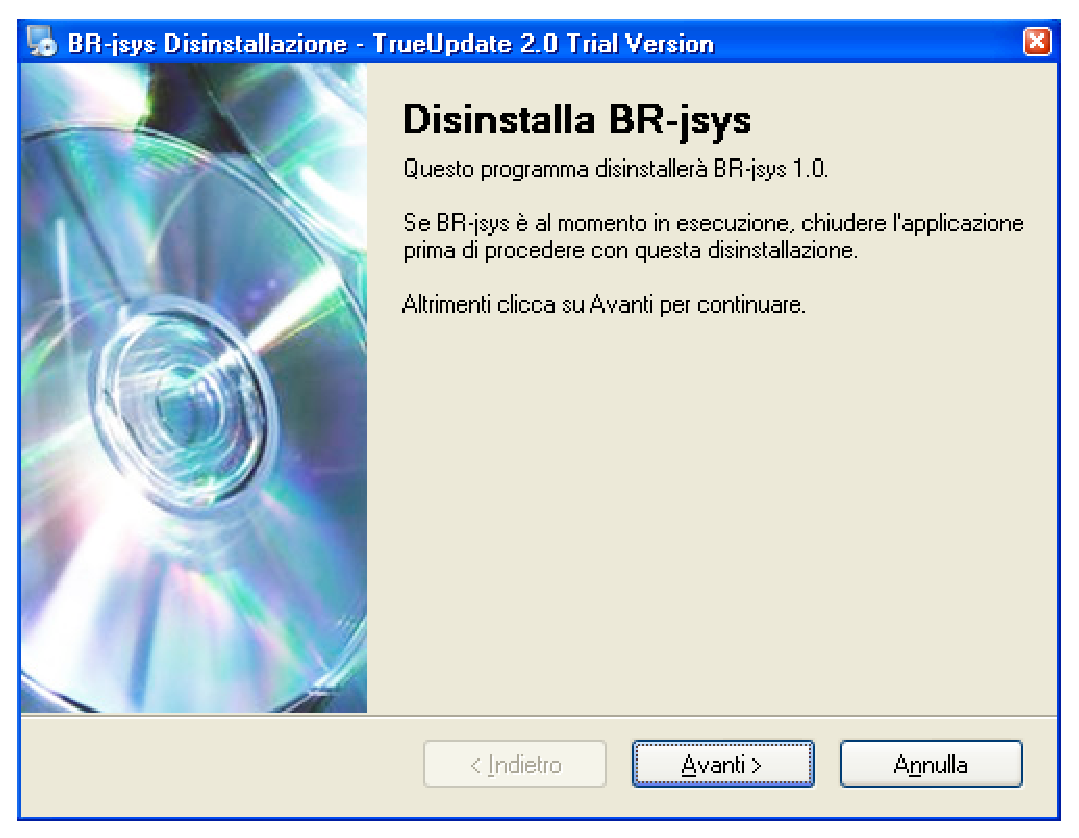
\includegraphics[width=0.8\textwidth]{manuale_utente/disinstalla_br-jsys_win.eps}\\
 figura 7.2: schermata iniziale
\end{center}
Al completamento cliccare su ``Fine''.
\begin{center}
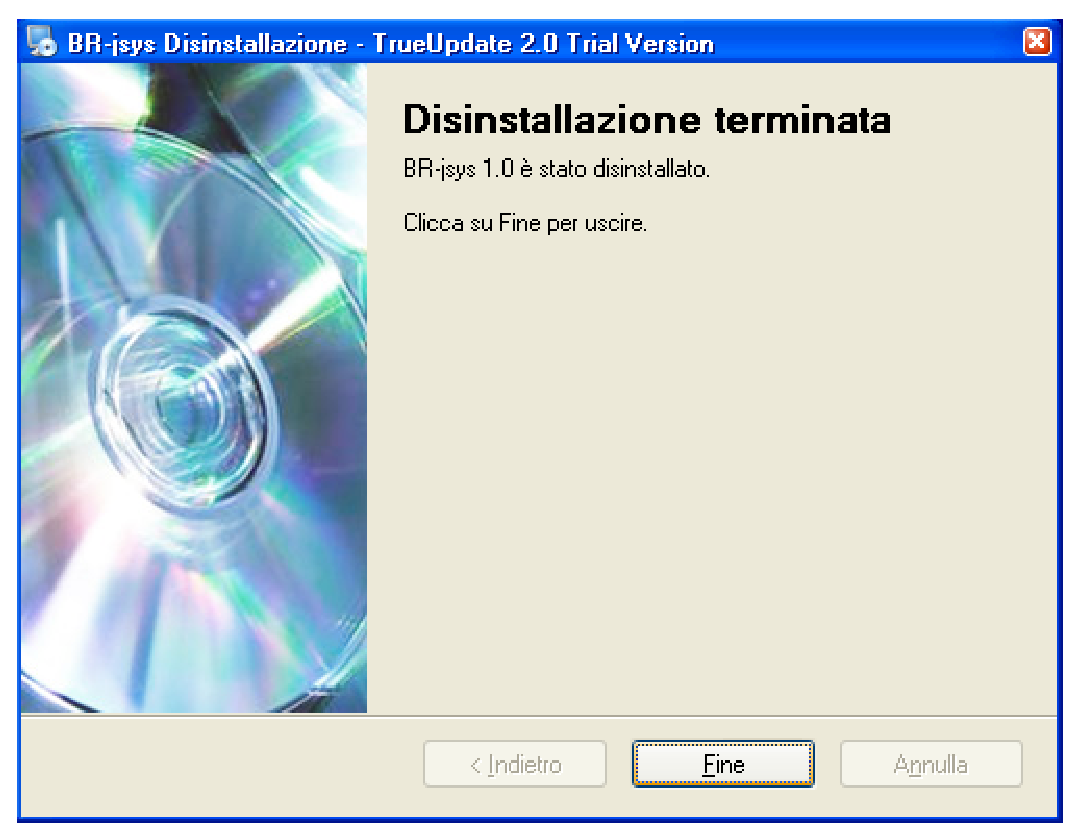
\includegraphics[width=0.8\textwidth]{manuale_utente/disinstalla_br-jsys_win1.eps}\\
 figura 7.2.1: schermata finale
\end{center}

\chapter{Messaggi d'errore}
\section{Come riportare problemi e malfunzionamenti}
Il prodotto software \`e dotato di un sistema di archiviazione svn. Tale archivio fornisce una sezione ``issues'' all'URL: \\ 
\href{http://code.google.com/p/br-jsys/issues/list}{http://code.google.com/p/br-jsys/issues/list}, che visualizza in qualsiasi momento la lista aggiornata di tutti i problemi e malfunzionamenti da noi riscontrati. Attraverso questo sistema ogni componente del gruppo potr\`a creare un ``new issue'', assegnandogli una priorit\`a che varier\`a a seconda della gravit\`a del problema. Ogni issue conterr\`a inoltre il nome dell'utente che lo ha aggiunto nella lista, oltre ad uno status (new, accepted, started, verified, etc...) che in qualsiasi momento ogni membro del gruppo potr\`a aggiornare. 

\newpage
\section{Messaggi di errore e loro significato}
\begin{table}[htbp]
\begin{tabular}{|p{2cm}|p{5cm}|p{5cm}|}
\hline
\textbf{ID:} & \textbf{Messaggio:} & \textbf{Descrizione:} \\ \hline
ERR00 & Autenticazione fallita & Nome utente e/o password non inseriti correttamente..\\ \hline
ERR & Server eXist spento. & Il server eXist non \`e avviato. \\ \hline
ERR & Campo dati regola non trovato. validazione interrotta! & Riferimento ad un campo dati sbagliato. La validazione viene interrotta. \\ \hline
ERR & Operazione non consentita: \textless tipo 1\textgreater\ != \textless tipo 2\textgreater\ : validazione interrotta & Errore tra tipi. Esecuzione di un'operazione di confronto tra due tipi diversi. La validazione viene interrotta. \\ \hline
ERR & Errore sintattico \textless tutta la business rule scritta fino all'errore\textgreater\ : validazione interrotta! & Errore di scrittura nella business rule. La validazione viene interrotta. \\ \hline
ERR & Testo regola gi\`a presente & La regola ha un nome gi\`a presente nel repository. Non verr\`a quindi inserita. \\ \hline
ERR & business rule non trovata! & La business rule cercata non \`e stata trovata nel \rp. \\ \hline
ERR & Repository vuoto! & Il repository \`e vuoto \\ \hline
\end{tabular} \\
\end{table}


\end{document}
